%%%%%%%%%%%%%%%%%%%%%%%%%%%%%%%%%
% 					ACSD Thesis Template v.2018a				 		%
%%%%%%%%%%%%%%%%%%%%%%%%%%%%%%%%%
% HowTo: https://acsd.etit.tu-chemnitz.de:5001/doku.php?id=start (TBD)
%----------------------------------------------------------------------------------------
%	PACKAGES AND OTHER DOCUMENT CONFIGURATIONS
%----------------------------------------------------------------------------------------

\documentclass[twoside, paper=a4, fontsize=12pt, german, open=right, colorpdf, dvipsnames]{scrreprt} 
% available options for this document class: 
% oneside/twoside: for one- or two-sided printing 
% english/german:
% dissertation: switches title page to dissertation style (submitted)
% final: works only in combination with "dissertation" option, switches titlepage style to final version (requires additional information)
% colorpdf: enebales full color mode (document will be greyscale if deleted - recommended for draft printing)

%%%%%%%%%%%%%%%%%%%%%%%%%%%%%%%%%%%%%%%%%
% Classicthesis Typographic Thesis
% Configuration File
%
% Important note:
% The main lines to change in this file are in the DOCUMENT VARIABLES
% section, the rest of the file is for advanced configuration.
%
%%%%%%%%%%%%%%%%%%%%%%%%%%%%%%%%%%%%%%%%%
%----------------------------------------------------------------------------------------
%	CHARACTER ENCODING
%----------------------------------------------------------------------------------------

\PassOptionsToPackage{utf8}{inputenc} % Set the encoding of your files. UTF-8 is the only sensible encoding nowadays. If you can't read äöüßáéçèê∂åëæƒÏ€ then change the encoding setting in your editor, not the line below. If your editor does not support utf8 use another editor!
\usepackage{inputenc}

\PassOptionsToPackage{listings, floatperchapter}{ACSDthesis}
% Available options: drafting parts manychapters floatperchapter listings

%----------------------------------------------------------------------------------------
%	USEFUL COMMANDS
%----------------------------------------------------------------------------------------

\newcommand{\ie}{i.\,e.}
\newcommand{\Ie}{I.\,e.}
\newcommand{\eg}{e.\,g.}
\newcommand{\Eg}{E.\,g.} 

\newcounter{dummy} % Necessary for correct hyperlinks (to index, bib, etc.)
\providecommand{\mLyX}{L\kern-.1667em\lower.25em\hbox{Y}\kern-.125emX\@}
\newlength{\abcd} % for ab..z string length calculation

%----------------------------------------------------------------------------------------
%	BIBLIOGRAPHY SETUP
%----------------------------------------------------------------------------------------

\usepackage{csquotes}
\PassOptionsToPackage{%
%backend=bibtex8, % Instead of bibtex
backend=biber,bibencoding=ascii,%
language=auto,%
style=numeric-comp,%
%%style=authoryear-comp, % Author 1999, 2010
%bibstyle=authoryear,dashed=false, % dashed: substitute rep. author with ---
sorting=nyt, % name, year, title
maxbibnames=10, % default: 3, et al.
%backref=true,%
natbib=true % natbib compatibility mode (\citep and \citet still work)
}{biblatex}
\usepackage{biblatex}

\DefineBibliographyStrings{english}{%
  mathesis = {Master's thesis},
}

\DefineBibliographyStrings{german}{%
  mathesis = {Masterarbeit},
  phdthesis = {Dissertation},
}

%----------------------------------------------------------------------------------------
%	PACKAGES
%----------------------------------------------------------------------------------------
 
%\PassOptionsToPackage{fleqn}{amsmath} % equations flushed left
\usepackage{amsmath, amsthm, amssymb, amsfonts} 
\DeclareMathOperator{\argmin}{argmin}

\PassOptionsToPackage{T1}{fontenc} % T2A for cyrillics
\usepackage{fontenc}
\usepackage{textcomp} % Fix warning with missing font shapes
\usepackage{scrhack} % Fix warnings when using KOMA with listings package  
\usepackage{xspace} % To get the spacing after macros right
\usepackage{mparhack} % To get marginpar right
\usepackage{fixltx2e} % Fixes some LaTeX stuff 
\PassOptionsToPackage{printonlyused, smaller}{acronym} % Include printonlyused in the first bracket to only show acronyms used in the text
\usepackage{acronym} % Nice macros for handling all acronyms in the thesis

\PassOptionsToPackage{pdftex}{graphicx}
\usepackage{graphicx} 
\usepackage{epsfig, epstopdf, tikz, calc}
\usepackage{enumerate, units, here}
\usepackage{multicol} % xcolor already loaded in style file
%\usepackage{todonotes}% um sich notizen zu machen wie z.b. dummie Bilder
%\usepackage{catchfile}
%\usepackage{autobreak} %kann in align umgebung seitenumbruch autom.

%----------------------------------------------------------------------------------------
%	FLOATS: TABLES, FIGURES AND CAPTIONS SETUP
%----------------------------------------------------------------------------------------

\usepackage{tabularx} % Better tables
\setlength{\extrarowheight}{3pt} % Increase table row height
\newcommand{\tableheadline}[1]{\multicolumn{1}{c}{\spacedlowsmallcaps{#1}}}
\newcommand{\myfloatalign}{\centering} % To be used with each float for alignment
\usepackage{caption}
\captionsetup{font=small, labelfont=bf}
\usepackage{subcaption}  

%----------------------------------------------------------------------------------------
%	CODE LISTINGS AND ALGOITHMS SETUP
%----------------------------------------------------------------------------------------

\usepackage{listings} 
%\lstset{emph={trueIndex,root},emphstyle=\color{BlueViolet}}%\underbar} % For special keywords
\lstset{language=[LaTeX]Tex,%C++ % Specify the language(s) for listings here
morekeywords={PassOptionsToPackage,selectlanguage},
keywordstyle=\color{RoyalBlue}, % Add \bfseries for bold
basicstyle=\small\ttfamily, % Makes listings a smaller font size and a different font
%identifierstyle=\color{NavyBlue}, % Color of text inside brackets
commentstyle=\color{BrickRed}\ttfamily, % Color of comments
stringstyle=\rmfamily, % Font type to use for strings
numbers=left, % Change left to none to remove line numbers
numberstyle=\scriptsize, % Font size of the line numbers
stepnumber=5, % Increment of line numbers
numbersep=8pt, % Distance of line numbers from code listing
showstringspaces=false, % Sets whether spaces in strings should appear underlined
breaklines=true, % Force the code to stay in the confines of the listing box
%frameround=ftff, % Uncomment for rounded frame
%frame=single, % Frame border - none/leftline/topline/bottomline/lines/single/shadowbox/L
belowcaptionskip=.75\baselineskip % Space after the "Listing #: Desciption" text and the listing box
}

\PassOptionsToPackage{linesnumbered, ruled}{algorithm2e}
\usepackage{algorithm2e}

%----------------------------------------------------------------------------------------

\usepackage{ACSDthesis} 

%----------------------------------------------------------------------------------------
%	USING DIFFERENT FONTS
%----------------------------------------------------------------------------------------

\usepackage[sfdefault]{roboto}
\usepackage{arev}

\newcommand{\bs}{\boldsymbol}
\newcommand{\bm}{\boldsymbol}

%\DeclareMathSizes{12}{11}{8.5}{7}
\linespread{1.1}
\setcapindent{1em}

%----------------------------------------------------------------------------------------
% RENEW DOTS
%----------------------------------------------------------------------------------------
\usepackage{accents}

\renewcommand*{\dot}[1]{%
  \begingroup
  \fontfamily{cmr}\selectfont{\accentset{\mbox{\bfseries\hspace{0.16ex}.}}{#1}}
  \endgroup
}

\renewcommand*{\ddot}[1]{%
  \begingroup
  \fontfamily{cmr}\selectfont{\accentset{\mbox{\bfseries\hspace{0.16ex}.\hspace{-0.25ex}.}}{#1}}
  \endgroup
}

%----------------------------------------------------------------------------------------
% USEFUL MAKROS
%----------------------------------------------------------------------------------------

\newcommand{\N}{\mathbb{N}}
\newcommand{\Z}{\mathbb{Z}}
\newcommand{\Q}{\mathbb{Q}}
\newcommand{\R}{\mathbb{R}}
\newcommand{\C}{\mathbb{C}}

 % Includes the file which contains all the document configurations and packages - make sure to edit this file

\addbibresource{thesis.bib} % The file housing your bibliography
%\addbibresource[label=ownpubs]{Self_Publications.bib} % Uncomment for optional self-publications

% Available Abbreviations: BA, MA, RP (Forschungsprojekt/Research Project) -> Dissertation is enabled via the ``dissertation'' option in documentclass (see above)
% The abbreviations are defined for both German and English
% You do not have to use the abbreviations but can enter the FULL thesis type manually 
\thesistype{Praktikumsbericht} 
\usetikzlibrary{patterns}
\finaldate{14. März 2024}

\title{Entwicklung und Implementierung einer automatisierten szenariobasierten Unit-Test Strategie für einen modellprädiktiven Pfadfolgeregler in einer GitLab CI Pipeline} % Titel der Arbeit

\subtitle{vorgelegt von} % Untertitel (falls vorhanden)

\author{Georg Ehrler} % Name des bearbeitenden Studenten

%%%%%%%% Personal Information for BA, MA, RP
\matrikel{521446}
\course{Energie- und Automatisierungssysteme}
%%%%%%%% Specific information for option "dissertation" %%%%%%%%
\dateofbirth{07.07.1999} % Geburtstag des bearbeitenden Studenten
\placeofbirth{Zwickau} % Geburtsort des bearbeitenden Studenten
%%%%%%%% Specific information for option "final" %%%%%%%% %%%%
\dateofsubmission{22.02.2022} 
\dateofdefence{33.03.3033} 
%%%%%%%%%%%%%%%%%%%%%%%%%%%%%%%%%%%%%%%

\supervisor{Francisco Moreno, M.Sc.} % Betreuer #1
\supervisor{Robert Ritschel, M.Sc. (IAV)} % Betreuer #2 (weitere Betreuer mit \supervisor{...} hinzufügen)

\examiner{Prof. Dr.\,-Ing. habil. Stefan Streif} % Prüfer (i.d.R. Prof. habil. Dr.\,-Ing. Stefan Streif); Für Dissertation: Gutachter (mehrere Gutachter möglich wie bei supervisor)

\company{IAV GmbH} % (optional) Name der Firma; Logo in figures/company_logo.pdf

%\hyphenation{Put special hyphenation here}
\sloppy

\begin{document}

\frenchspacing % Reduces space after periods to make text more compact
\raggedbottom % Makes all pages the height of the text on that page

%----------------------------------------------------------------------------------------
%	PRE-CONTENT THESIS PAGES
%----------------------------------------------------------------------------------------

\pagenumbering{roman} % Roman page numbering prior to the start of the thesis content (i, ii, iii, etc)
\pagestyle{plain} % Suppress headers for the pre-content pages
\maketitle
\pagenumbering{Roman}

% \setcounter{page}{1}
\pdfbookmark[1]{Kurzfassung}{Kurzfassung} % Bookmark name visible in a PDF viewer
\chapter*{\bfseries Kurzfassung} %mit * bedeutet, nicht im Inhaltsverzeichnis
\thispagestyle{empty}

kurze Zusammenfassung, tbd.

\cleardoublepage

\chapter*{\bfseries Abstract} %mit * bedeutet, nicht im Inhaltsverzeichnis
\thispagestyle{empty}

Short summary, tbd.

\cleardoublepage%%Abstract
% Table of Contents with respective options
\refstepcounter{dummy}
\pdfbookmark[1]{\contentsname}{tableofcontents} % Bookmark name visible in a PDF viewer
\setcounter{tocdepth}{2} % Depth of sections to include in the TOC - currently up to subsections
\setcounter{secnumdepth}{3} % Depth of sections to number in the text - currently up to subsubsections
\tableofcontents
\thispagestyle{empty}
\cleardoublepage % fix first bookmark after toc%%Inhaltsverzeichnis (including tocdepth & secnumdepth options)
% \refstepcounter{dummy}
\addcontentsline{toc}{chapter}{Symbolverzeichnis}
%\pdfbookmark[1]{Symbolverzeichnis}{Symbolverzeichnis} % Bookmark name visible in a PDF viewer % not needed because its added to toc and therfore shows up as a bookmark

\allowdisplaybreaks
\chapter*{\bfseries Symbolverzeichnis}
\thispagestyle{empty}
\vspace{-.5em} % Fix Notation top margin! Do not edit or delete!!!
\begin{tabular}{@{} p{\figurelabelwidth} @{} p{\textwidth-\figurelabelwidth}}
$k$ 				 & time instant for the high level prediction model\\
$\kappa$ 			 & time instant for the low level prediction model\\
$\bm{x}$	  		 & state vector\\
$\bm{u}$		  	 & input vector\\
$\bm{y}$		  	 & output vector\\
$\bm{\bar{x}}$  	 & predicted state vector\\
$\bm{\bar{u}}$  	 & predicted input vector\\
$\bm{\bar{y}}$  	 & predicted output vector\\
$\bm{x}_{i}$	 	 & state vector of the $i^{\text{th}}$ subsystems\\
$\bm{u}_{i}$	 	 & input vector of the $i^{\text{th}}$ subsystems\\
$\bm{x}_{\max}$ 	 & upper bound for the state\\
$\bm{x}_{\min}$	 & lower bound for the state\\
$\bm{u}_{\max}$	 & upper bound for the input\\
$\bm{u}_{\min}$ 	 & lower bound for the input\\
$\bm{N}$	 	 	 & length of the prediction horizon\\
$\bm{I}$	 	 	 & identity matrix of appropriate dimension\\
$\mathcal{X}$	  	 & state sequence of the prediction\\
$\mathcal{U}$	 	 & input sequence of the prediction\\
$\mathbb{R}$	  	 & set of real numbers\\
$\mathbb{R}^{n}$& set of $n$-dimensional vectors of real numbers\\
$\mathbb{R}^{n \times m}$ & set of $n \times m$ matrices of real numbers\\
$\mathbb{U}$	  	 & set of feasible inputs\\
$\mathbb{X}$	  	 & set of feasible states\\
\end{tabular}                   
\cleardoublepage

%%Symbolverzeichnis
% \refstepcounter{dummy}
\addcontentsline{toc}{chapter}{Abkürzungsverzeichnis}
%\pdfbookmark[1]{Abkürzungsverzeichnis}{Abkürzungsverzeichnis} % Bookmark name visible in a PDF viewer % not needed because its added to toc and therfore shows up as a bookmark

\begingroup 
\let\clearpage\relax
\let\cleardoublepage\relax
\let\cleardoublepage\relax

\chapter*{Abkürzungsverzeichnis}
\thispagestyle{empty}
\vspace{-.5em} % Fix LoA top margin! Do not edit or delete!!!
\begin{tabular}{@{} p{\figurelabelwidth} @{} p{\textwidth-\figurelabelwidth}}
\textbf{MPC} & Model Predicitive Control, modellprädiktive Regelung\\
\textbf{MPFC} & Model Predicitive Path Following Control, modellprädiktive Pfadfolgeregelung\\
\textbf{ACC} & Adaptive Cruise Control, Abstandsregeltempomat\\
\textbf{KPI} & Key Performance Indicator, Leistungskennzahl\\
\textbf{CI} & Continuous Integration, kontinuierliche Integration\\
\end{tabular}                
\endgroup
\cleardoublepage%%Symbolverzeichnis
\addtocontents{lof}{\protect\vspace{-.9em}} % Fix LoF top margin! Do not edit or delete!!!
\listoffigures\addcontentsline{toc}{chapter}{Abbildungsverzeichnis}%%Abbildungsverzeichnis
\thispagestyle{empty}

\cleardoublepage
\pagestyle{scrheadings} % Show chapter titles as headings
\pagenumbering{arabic} % Arabic page numbering for thesis content (1, 2, 3, etc)
\cleardoublepage % Avoids problems with pdfbookmark
\renewcommand*{\arraystretch}{1}

%----------------------------------------------------------------------------------------
%	THESIS CONTENT - CHAPTERS
%----------------------------------------------------------------------------------------
\chapter{Einleitung} \label{chap:Einleitung}
\thispagestyle{empty}
Gesetzliche Bestimmungen zur Erhöhung der Sicherheit von sowohl den Insassen eines Fahrzeugs als auch anderer Verkehrsteilnehmer haben in den letzten Jahrzehnten zu einer signifikanten Senkung der Mortalitätsrate bei Verkehrsunfällen beigetragen.
\begin{figure}[H]
    \centering
    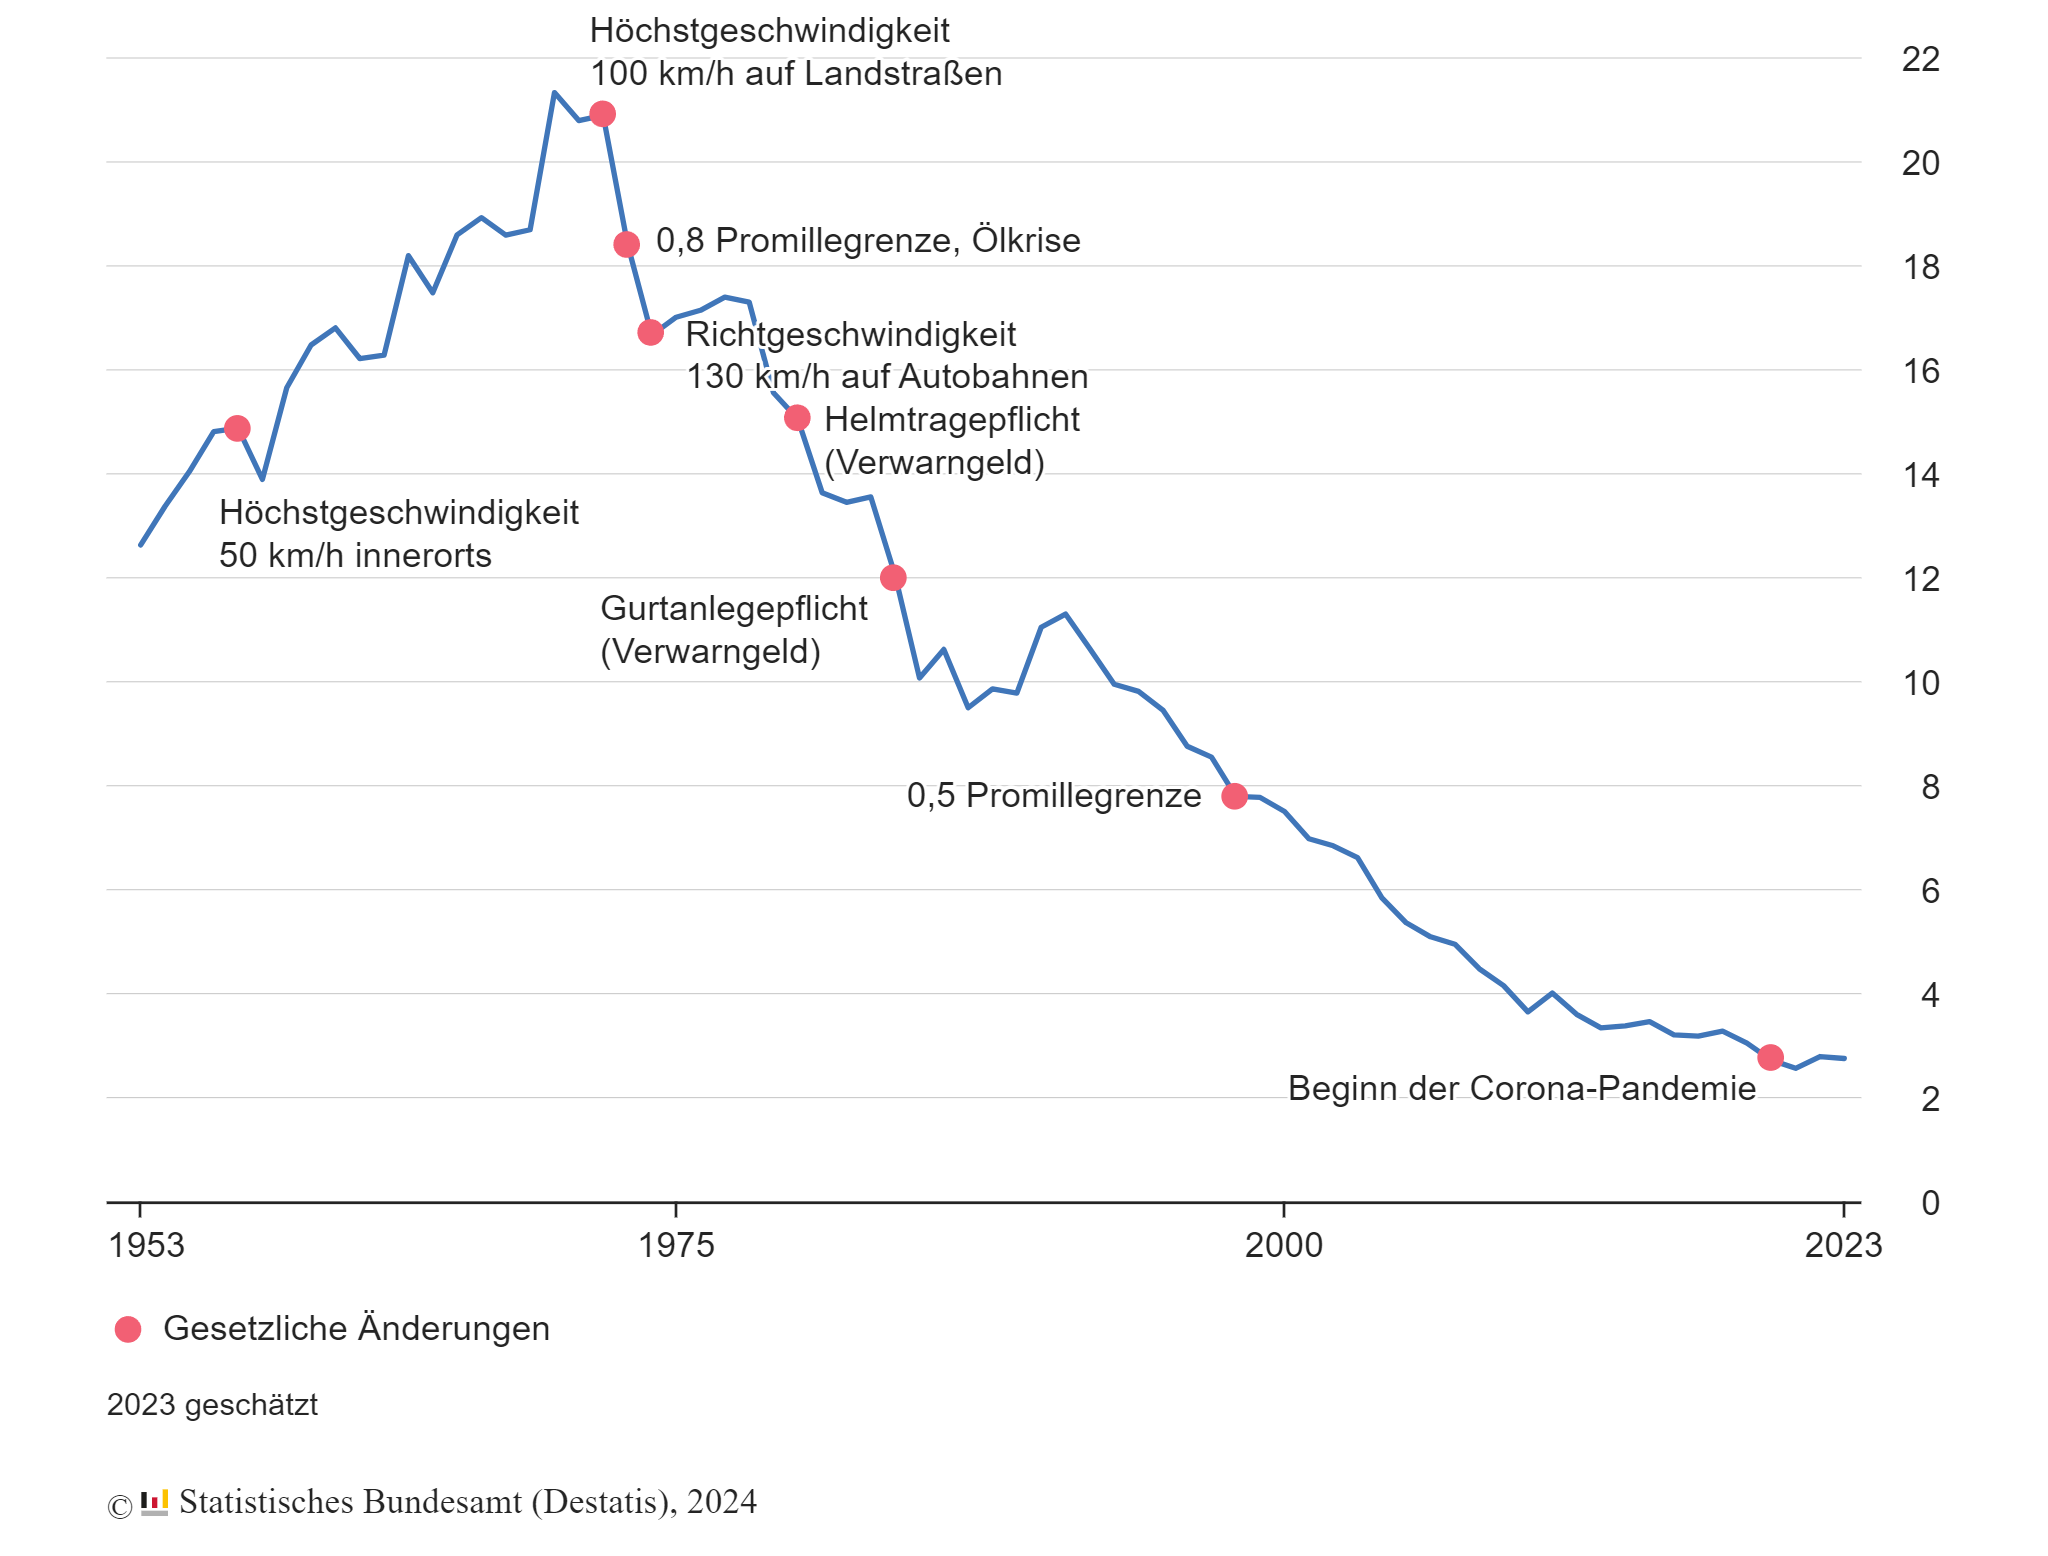
\includegraphics[width=0.9\textwidth]{figures/1_Einleitung/verkehrsunfaelle-getoetete-jahr.png}
    \caption{Bei Verkehrsunfällen Getötete pro Jahr in Tausend \cite{StBA2021}}
    \label{fig:Statistik_Tote}
\end{figure}
\noindent Im Jahr 2021 gab es über 250.000 Unfälle mit Personenschaden auf deutschen Straßen. In 88 \% der Fälle ist die Ursache auf ein Fehlverhalten der Fahrzeugführer zurückzuführen \cite{StBA2021}. Der Einsatz von automatisierten Fahrzeugen kann zu einem weiteren Rückgang der in Abbildung \ref{fig:Statistik_Tote} gezeigten Statistik führen, indem es den Fahrer durch Einsatz von intelligenten Assistenzsystemen unterstützt oder die menschliche Fehlerkomponente gänzlich beseitigt, indem ein Fahrzeug vollständig autonom fährt.

Um die Sicherheit der Fahrzeuge zu gewährleisten, muss sowohl das Gesamtsystem, als auch alle Teilsysteme intensiv getestet werden. Eines dieser Teilsysteme für das hochautomatisierte Fahren ist die Regelung der Längs- und Querführung des Fahrzeugs. Bei der IAV\footnote{\url{https://www.iav.com/}} geschieht dies durch einen modellprädiktiven Pfadfolgeregler.\bigskip

\noindent\textbf{Aufgabenstellung}\smallskip

\noindent Im Rahmen des Praktikums soll eine automatisierte Teststrategie für einen modellprädiktiven Pfadfolgeregler (engl. Model Predictive Pathfollowing Control, MPFC) konzeptioniert und implementiert werden.

Modellprädiktive Regler (engl. Model Predictive Control, MPC) eignen sich hervorragend für die Vorhersage und Regelung dynamischer Systeme, da sie auf Störungen im Betrieb gut reagieren können, weshalb sie in vielen Industriezweigen, einschließlich der Automobilindustrie, Anwendung finden \cite{adamy2014}. Im Bereich des hochautomatisierten Fahrens können mithilfe von MPC in Echtzeit Fahrentscheidungen, die sowohl sicherheits- als auch komfortrelevante Anforderungen erfüllen, getroffen werden. Um die Sicherheit und Zuverlässigkeit des Systems sicherzustellen, sollen realitätsnahe Fahrszenarien ermittelt und anhand von festgelegten Key Performance Indicators (KPIs) bewertet werden. Dieser Prozess soll automatisiert in einer CI Pipeline ablaufen.\medskip

\noindent Es sind die folgenden Teilaufgaben umzusetzen:
\begin{itemize}
    \item Konzeptentwicklung für das automatisierte, szenariobasierte Testen der MPFC unter Verwendung der bestehenden Simulationsumgebung
    \item Definition und Parametrierung geeigneter Fahrszenarien
    \item Definition von KPIs zur Beurteilung der Leistung der Regelung
    \item Einbindung in eine GitLab CI Pipeline
    \item Dokumentation der Ergebnisse
\end{itemize}

\chapter{Grundlagen} \label{chap:Grundlagen}
\thispagestyle{empty}
In diesem Kapitel wird zunächst eine Einführung in alle Themenbereiche gegeben. Insbesondere wird der modellprädiktive Pfadfolgeregler näher erläutert, um ein besseres Systemverständnis zu erlangen. Außerdem wird auf  Strategien für das Überprüfen von Software und Testabläufe, speziell in der Automobilindustrie, näher eingegangen und ein Einblick in aktuelle Softwarentwicklungsabläufe gegeben. 
\section{Modellprädiktive Pfadfolgeregelung} \label{sec:MPFC}
\subsection{Modellprädiktive Regelung}
Die modellprädiktive Regelung (engl. Model Predictive Control, MPC) ist ein Verfahren zur Regelung von dynamischen Systemen. Dabei wird ein mathematisches Modell des Systems erstellt und zur Vorhersage der zukünftigen Systemzustände verwendet. Das prädizierte Systemverhalten wird dann verwendet, um ein Optimalsteuerungsproblem (engl. Optimal Control Problem - OCP) zu lösen und die optimale Eingabe zu finden um das System in einen gewünschten Zustand zu bringen.
\begin{figure}
    \centering
    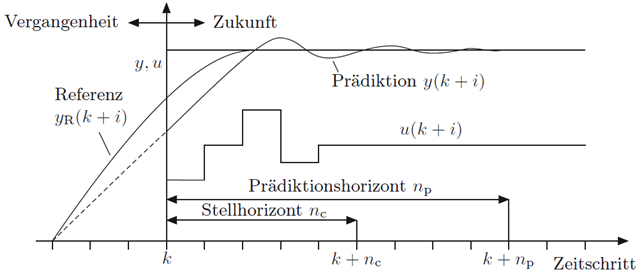
\includegraphics[width=0.7\textwidth]{figures/2_Grundlagen/MPC_Diagramm.png}
    \caption{Ablauf einer modellprädiktiven Regelung \cite{adamy2014}}
    \label{fig:MPC}
\end{figure}
Der Ablauf einer modellprädiktiven Regelung, wie in Abbildung \ref{fig:MPC} zu sehen, kann in drei Punkte unterteilt werden \cite{camacho2013model}:
\begin{enumerate}
    \item Mithilfe eines Modells wird der Ausgang eines Systems für $k+n_{p}$ Zeitschritte (Prädiktionshorizont) vorausgesagt. Die Prädiktion basiert sowohl auf den vergangenen Ein- und Ausgängen als auch auf den zukünftigen Eingaben über die Länge des Stellhorizonts $n_{c}$
    \item Die Stellgrößensequenz $u$ wird berechnet. Dabei wird eine Kostenfunktion minimiert, welche so gewählt wird, dass sich ein gewünschtes Systemverhalten einstellt. Der Stellaufwand wird in der Regel in der Kostenfunktion mit berücksichtigt. Ebenfalls können Beschränkungen, von z.B. den Eingangsgrößen, berücksichtigt werden. Für jeden Zeitschritt wird so das OCP gelöst.
    \item Das erste Element des Stellhorizonts wird auf das System angewendet. Stell- und Prädiktionshorizont verschieben sich um einen Zeitschritt in die Zukunft. Der Zyklus beginnt von vorn. 
\end{enumerate}
\subsection{Pfadfolgeregelung}
Die Implementierung der Pfadfolgeregelung für die in diesem Praktikum eine Teststrategie implementiert werden soll, ist in \ref{fig:MPFC_Schema} dargestellt. Als Eingänge dienen der MPFC eine Sollgeschwindigkeit, Pfaddaten, Fahrzeugzustände, vorgegebene Beschränkungen und ein Modell. Daraus werden eine Sollbeschleunigung und eine Solllenkradwinkelgeschwindigkeit berechnet.

%TODO: den nochmal neu Schreiben
Die Grundidee ist in \cite{Faulwasser2009} beschrieben: Der Regelungsalgorithmus soll einem Referenzpfad folgen, es ist jedoch nicht vorgegeben, wann das System an welcher Stelle des Pfades sein muss. Die Geschwindigkeit entlang des Pfades kann also als ein zusätzlicher Freiheitsgrad verwendet werden. Durch eine Modifikation des Ansatzes aus \cite{Faulwasser2009} kann eine gewünschte Geschwindigkeit dem Pfad zugeordnet werden, die Fahrzeuggeschwindigkeit wird auf die Pfadgeschwindigkeit konvergieren, die Einhaltung dieser ist allerdings nicht sichergestellt. Ein konvergieren des Fahrzeug auf den Pfad und die Einhaltung von Beschränkungen wird garantiert \cite{ritschel2019}.
%TODO:

Eine Methode zur Ermittlung geeigneter Parameter für das Optimierungsproblem der Pfadfolgeregelung ist in \cite{math11020465} dokumentiert. Darin steht die Erhöhung der Sicherheit und des Fahrkomfort im Fokus. Durch eine bayessche Optimierung werden Parameterwerte, welche eine gutes Verfolgen der Pfadgeschwindigkeit, geringe Abweichung vom Pfad und möglichst geringe laterale sowie longitudinale Beschleunigungen erzeugen, gefunden. Letzteres ist ein großer Faktor wenn es um Fahrkomfort geht, wie  auch \cite{BELLEM201890} verdeutlicht.
\begin{figure}[H]
    \centering
    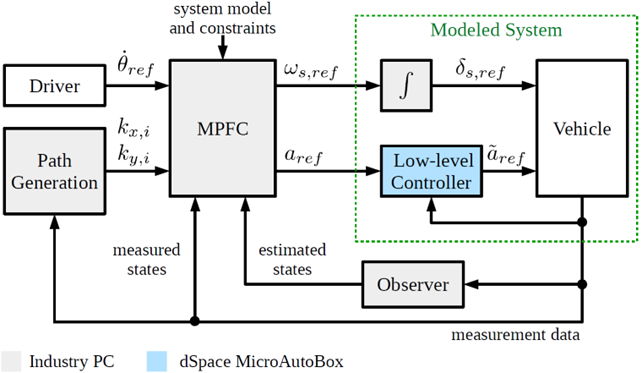
\includegraphics[width=0.7\textwidth]{figures/2_Grundlagen/MPFC_Schema.png}
    \caption{schematischer Aufbau der MPFC \cite{ritschel2019}}
    \label{fig:MPFC_Schema}
\end{figure}
    
\section{Szenariobasiertes Testen im Automobilbereich} \label{sec:SoftwaretestsAutomobil}

Um ein autonomes Fahrsystem zu realisieren und Sicherheit zu gewährleisten sind ausgiebige Test- und Verifikationsprozesse erforderlich. Dabei ist es nicht mehr ausreichend, Testdaten durch reale Testfahrten auf der Straße zu sammeln. Ein großer Anteil der Daten ist schlichtweg uninteressant, da keine kritischen Fahrsituation auftreten. Es bietet sich daher an, in einer Datenbank die kritischen Szenarien zu erfassen und für spätere Verifikationsprozesse wieder heranzuziehen \cite{Nalic2020}.

Um Szenarien zu beschreiben und in eine Datenbank einordnen zu können müssen diese klassifiziert werden. Eine Möglichkeit dafür ist die Einteilung nach Informationslevel \cite{Nalic2020}\cite{Bagschik2018}.
\begin{figure}[H]
    \centering
    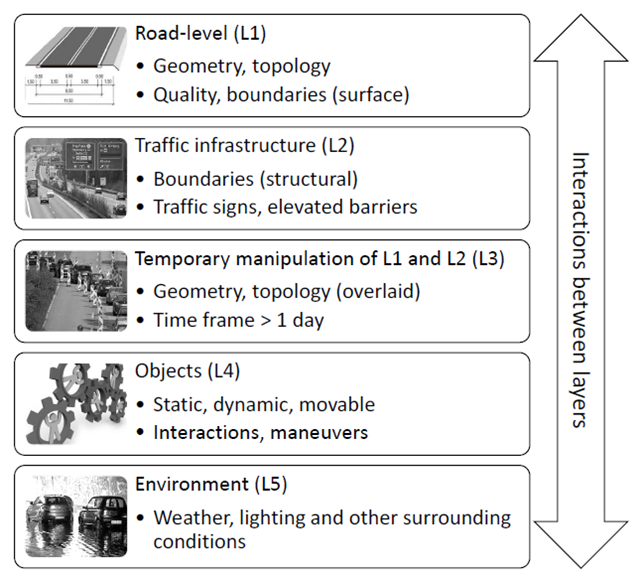
\includegraphics[width=0.5\textwidth]{figures/2_Grundlagen/layer_model.png}
    \caption{Einteilung des Informationsgehalts eines Szenarios nach Schichten \cite{Bagschik2018}}
    \label{fig:layer_model}
\end{figure}
Die erste Ebene definiert dabei grundlegende Eigenschaften der Straße, wie etwa deren Beschaffenheit oder Grenzen. Die nächste Ebene fügt Infrastrukturobjekte wie Straßenschilder hinzu. Ebene drei enthält Informationen über temporäre Veränderungen der darunterliegenden Ebenen. Ebene vier fügt einem Szenario statische und dynamische Objekte wie andere Verkehrsteilnehmer und Manöverplanung hinzu. Zum Schluss können noch Umweltfaktoren eingefügt werden \cite{Bagschik2018}.

Eine weitere Klassifizierungsmöglichkeit ist nach dem Detailgrad, wie es in Abbildung \ref{fig:scenario_level} \cite{Nalic2020}\cite{menzel2018scenarios}. Zunächst werden funktionale Szenarios beschrieben. Diese können einfach mit Worten beschrieben werden und enthalten noch keine Information über die Parameter. In einem ersten Abstrahierungsschritt werden diese zu logischen Szenarios. Hier wurden Parameter identifiziert und Grenzen für diese festgelegt. Um ein konkretes Szenario zu erhalten muss für jeden Parameter ein Wert ausgewählt werden. Theoretisch ermöglicht dies eine unendliche Anzahl an konkreten Szenarios, welche aus lediglich einem funktionalen Szenario erstellt werden können. Selbst bei rein simulativen Tests ist das nicht umsetzbar und muss reduziert werden \cite{menzel2018scenarios}.
\begin{figure}
    \centering
    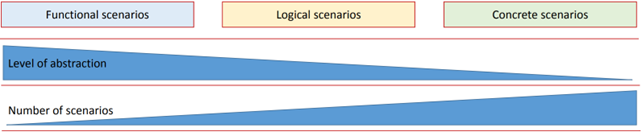
\includegraphics[width=0.9\textwidth]{figures/2_Grundlagen/scenario_level.png}
    \caption{Erhöhung der Anzahl an Szenarios mit zunehmener Konkretisierung der Szenarien \cite{menzel2018scenarios}}
    \label{fig:scenario_level}
\end{figure}

\section{Softwartests und CI/CD} \label{sec:CICD}

Ein geeignetes Testmanagement erhöht die Qualität einer Software maßgeblich. Ein Testprozess läuft in der Regel nach dem in Abbildung \ref{fig:testprozess} dargestellten Schema ab. Für den Testprozess exitisieren die Normen IEEE 829 und ISO-Standard 9126. Das International Software Testing Qualifications Board (ISTQB) arbeitet auf Grundlage dieser Normen an der Standardisierung von Systemtests \cite{witte2019testmanagement}.
\begin{figure}
    \centering
    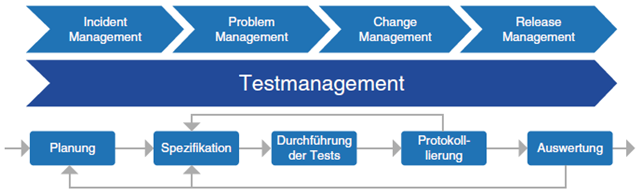
\includegraphics[width=0.9\textwidth]{figures/2_Grundlagen/testprozess.png}
    \caption{Ablauf eines Testprozesses \cite{witte2019testmanagement}}
    \label{fig:testprozess}
\end{figure}

Eine Möglichkeit Testprozesse Durchzuführen steckt hinter den Schlagworten Continuous Integration (CI) und Continuous Deployment (CD). Darunter versteht sich ein Prozess zum entwickeln, testen und freigeben von Software unter Nutzung von Versionsverwaltungssoftware wie er in Abbildung \ref{fig:ci-cd-flow-desktop} dargestellt ist. Wenn ein Entwickler in einem Softwaremodul Änderungen veranlasst, läuft ein automatischer Testprozess ab. Dieser ist typischerweise in Stages unterteilt, in Abbildung \ref{fig:ci-cd-flow-desktop} sind diese BUILD, TEST, MERGE. Werden darin keine Fehler in der Software gefunden werden die Änderungen eines Moduls zusammen mit den Änderungen an allen Modulen zusammengefasst und und somit die gesamte Software auf den aktuellen Stand gebracht (Continuous Delivery). Werden für die Gesamtsoftware ebenfalls keine Fehler gefunden kann eine neue Softwareversion zum Kunden gebracht werden (Continuous Deployment). Dieser Testprozess läuft in der Regel automatisch ab und veringert die Anzahl an Fehlern in Software \cite{redhat2024}.
\begin{figure}
    \centering
    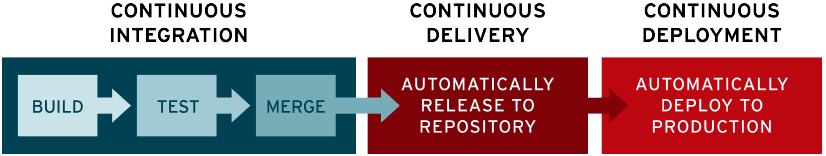
\includegraphics[width=0.9\textwidth]{figures/2_Grundlagen/ci-cd-flow-desktop.png}
    \caption{Ablauf eines CI/CD Prozesses \cite{redhat2024}}
    \label{fig:ci-cd-flow-desktop}
\end{figure}
\chapter{Implementierung} \label{chap:Implementierung}
\thispagestyle{empty}
In diesem Kapitel werden die implementierten Funktionen und Klassen dokumentiert. Dabei wird zunächst der Aufbau und der Ablauf von klassenbasierten Unit-Tests aus dem MATLAB\textsuperscript{\textregistered} Unit-Test Framework beschrieben und wie sich damit ein Konzept für das szenariobasierte Testen realisieren lässt. Weiterhin wird der Ablauf eines Testskriptes erläutert und auf die Einbindung in die GitLab CI-Pipeline eingegangen. Außerdem werden die KPIs zur Bewertung der Simulationsergebnisse eingeführt.

\section{Anforderungen} \label{sec:Anforderungen}
Aus der Aufgabenstellung ergeben sich bereits die wichtigsten Anforderungen. Zunächst soll ein Konzept für das Testen der MPFC, basierend auf dem MATLAB\textsuperscript{\textregistered} Unit-Test Framework, erarbeitet werden. Dafür muss eine geeignete Struktur gefunden werden, welche eine automatisierte Ausführung ermöglicht und Variationen von sowohl Testparametern (bspw. Initialgeschwindigkeiten) als auch MPC-Parametern (bspw. Gewichte der Kostenfunktion) leicht umzusetzen sind. 

Es sollen Szenarien gefunden und parametriert werden, welche für den Regelungsalgorithmus eine Herausforderung darstellen und so das Verhalten in kritischen Situationen getestet werden kann.

Um die Simulationsergebnisse bewerten zu können, sollen geeignete Kriterien bestimmt werden, die sowohl die Sicherheit als auch den Komfort der gefundenen Lösung bewerten. Diese Kriterien werden im weiteren Verlauf als KPIs bezeichnet. 

Ein KPI ist ein Grenzwert für eine messbare Größe in den Simulationsdaten. Wird dieser Grenzwert durch ein Über- bzw. Unterschreiten verletzt, führt dies zu einem negativen Ergebnis für den Testlauf.

Aus den Testergebnissen soll abschließend ein Bericht erstellt werden, welcher dem Entwickler übersichtlich mögliche Fehlschläge aufzeigt.

\section{Simulationsumgebung} \label{sec:Simulationsumgebung}
Die Simulationsumgebung und der Regelungsalgorithmus sind bereits in vorherigen Entwicklungsprojekten bei der IAV entstanden und sind in MATLAB\textsuperscript{\textregistered}/Simulink implementiert. Aus den Streckeninformationen wird ein gewünschter Pfad mit einer Zielgeschwindigkeit generiert und straßenähnlich dargestellt. Darauf wird die tatsächliche und prädizierte Bewegung des Fahrzeugs abgebildet.  
In Abbildung \ref{fig:Simulation_Strecke} ist dieser generierte Live-Plot zu sehen.
\begin{figure}[ht]
    \centering
    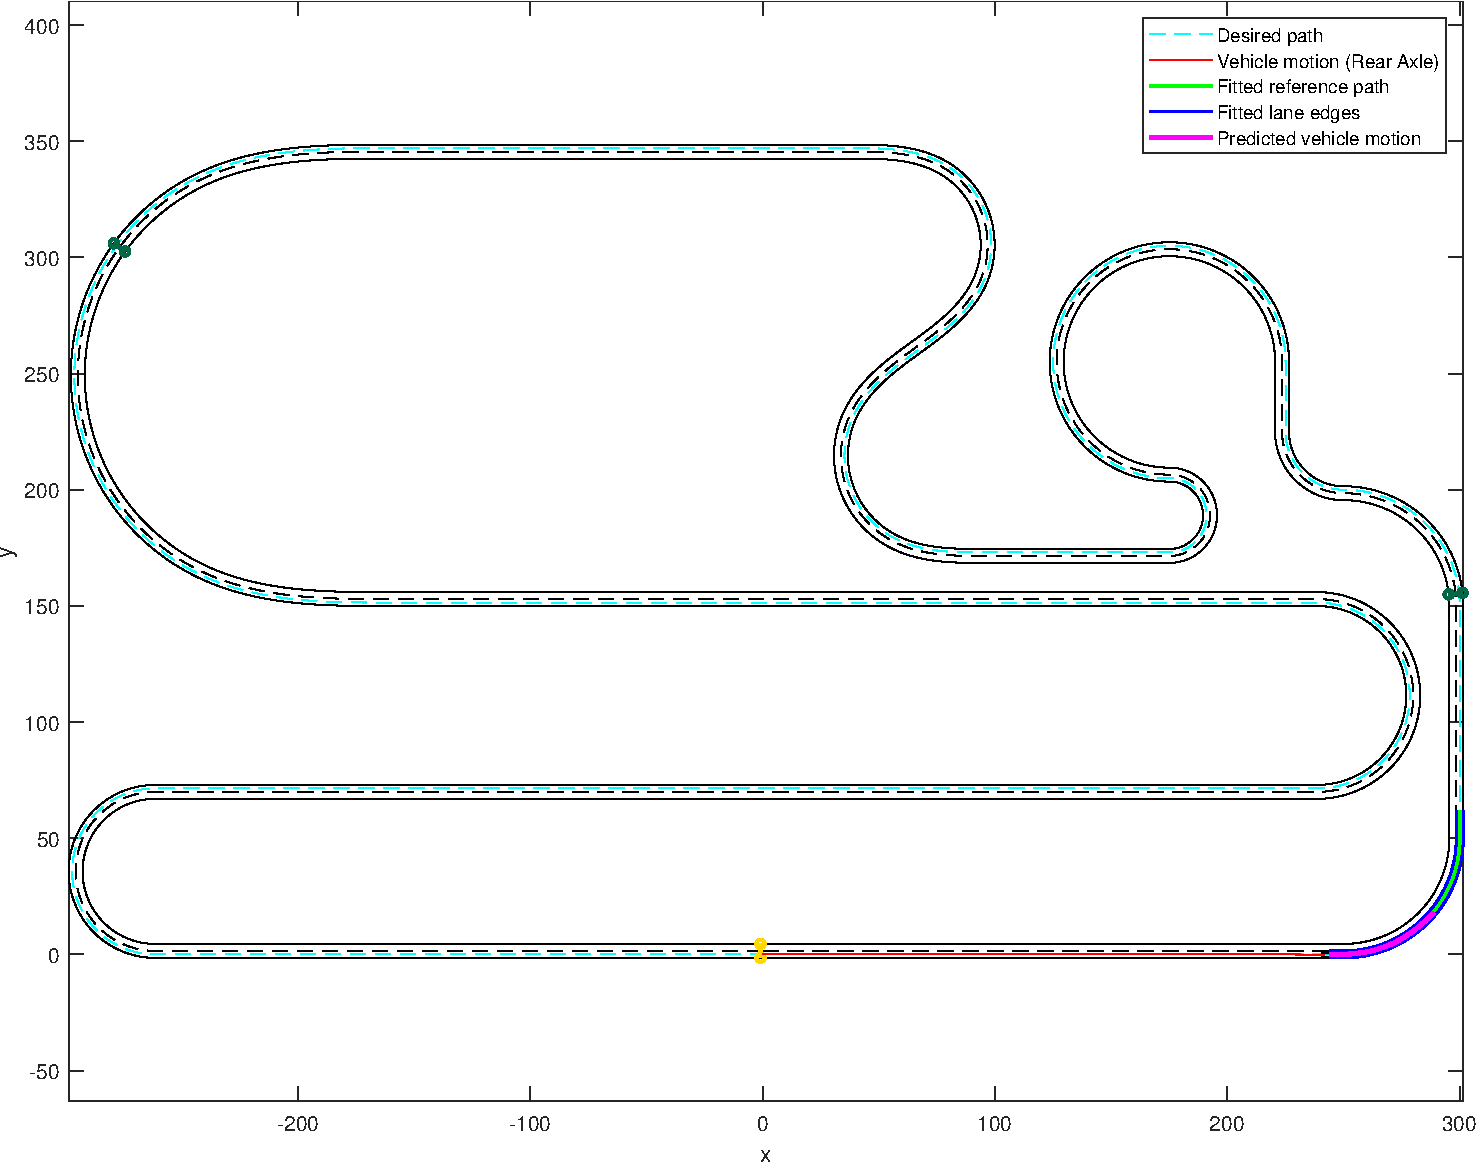
\includegraphics[width=0.6\textwidth]{figures/3_Implementierung/simulationsumgebung.pdf}
    \caption{Beispiel einer komplexen Simulationsstrecke}
    \label{fig:Simulation_Strecke}
\end{figure}

\section{MATLAB\textsuperscript{\textregistered} Unit-Test Framework} \label{sec:MatlabUnitTest}
MATLAB\textsuperscript{\textregistered}, in der für dieses Praktikum verwendeten Version 2022a und 2023b, stellt in der Basiskonfiguration ein umfangreiches Framework für die Implementierung von Unit-Tests zur Verfügung \cite{matlabTest}. Eine Verwendung dieser Funktionalität für das Testen der MPFC liegt nahe, da diese vollständig in diesem Programm implementiert ist.

Grundsätzlich gibt es drei Arten von Testabläufen: skriptbasierte, funktionsbasierte und klassenbasierte Tests. Diese unterscheiden sich vornehmlich im Funktionsumfang, wobei klassenbasierte Tests am umfangreichsten sind. Diese bieten als einzige die Möglichkeit, Tests durch externe Parameter zu parametrisieren. Da dies eine direkte Anforderung an das zu entwickelnde Konzept ist, wurde sich für die Verwendung der klassenbasierten Tests entschieden \cite{matlabTest}.

Das grundlegende Element dieses Frameworks ist der \textit{test case}. In diesem wird über \textit{assertions}, dies sind meist logische Operationen, festgestellt, ob sich ein System im Normbereich befindet. Ist dies nicht der Fall, wird der Test abgebrochen und als fehlgeschlagen angesehen.

Um sicherzustellen, dass sich das \textit{System Under Test (SUT)} vor einem Test in einem definierten Zustand befindet und vorherige Programmausführungen keine Auswirkungen auf die Testergebnisse haben, wird über \textit{test fixtures} dieser definierte Zustand hergestellt \cite{xUnitpatterns}. Bei klassenbasierten Tests gibt es mehrere Stellen, an denen initiale Zustände hergestellt werden können. Mithilfe der Setup-Methoden können Voraussetzungen für mehrere Klassen (shared fixtures), für alle Testfälle einer Klasse (testclass setup) initial oder vor Ausführung jedes einzelnen Testfalls (testmethod setup) geschaffen werden.

Eine \textit{test suite} ist eine Sammlung von Testfällen, welche die gleichen Initialzustände teilen. Da in der späteren Implementierung eine Testsuite immer aus lediglich einer Testklasse erstellt wird, bezeichnen Testsuite und Testklasse hier das gleiche Objekt. 

Bei klassenbasierten Tests ist es zudem möglich, externe Parameter in die Testklasse zu laden. Diese können als Testparameter, Testinitialisierungsparameter oder Klasseninitialisierungsparameter übergeben werden. Abhängig davon, welche Parametertypen und wie viel Variationen definiert sind, werden Testfälle und die verschiedenen Setup-Methoden mehrmals ausgeführt. 
% Eine eigene Darstellung des Ablaufs einer Testklasse ist in Abbildung \ref{fig:Testklassen_Ablauf} zu sehen. 

% \begin{figure}[ht]
%     \centering
%     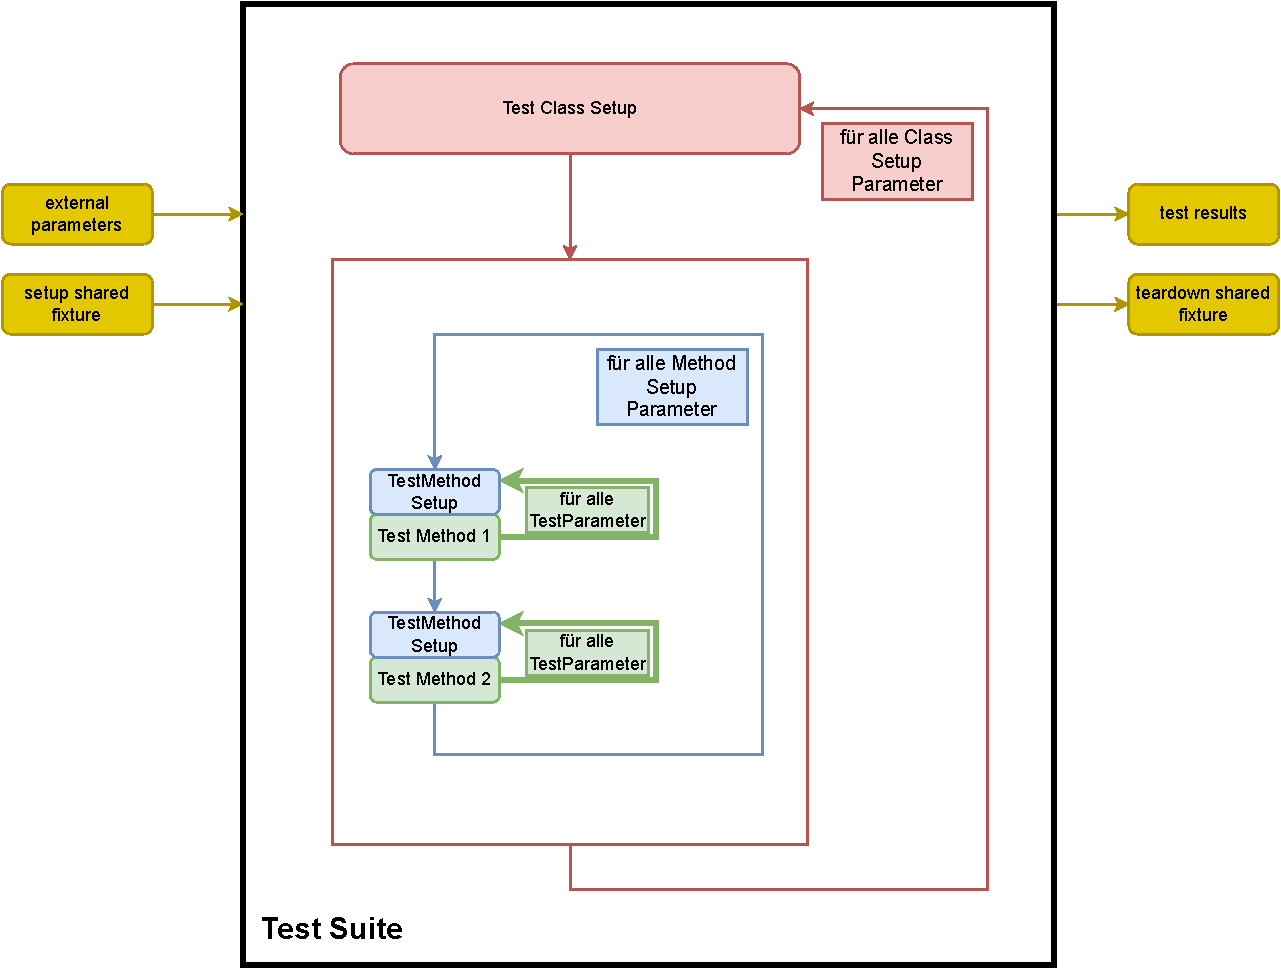
\includegraphics[width=0.75\textwidth]{figures/3_Implementierung/Testklassen_Ablauf.drawio.pdf}
%     \caption{Ablauf von klassenbasierten Tests}
%     \label{fig:Testklassen_Ablauf}
% \end{figure}

Ein konfigurierbarer \textit{test runner} führt die Tests aus. Das Framework sorgt selbstständig dafür, dass die notwendigen Setup-Methoden an den richtigen Stellen ausgeführt werden.

Für die Darstellung der Testergebnisse existiert ein \textit{test result formatter}, welcher die Ergebnisse in vielen Formaten, beispielsweise PDF oder XML, aufbereitet.

Die objektorientierte Natur von MATLAB\textsuperscript{\textregistered} und dem Unit-Test Framework ermöglichen zusätzlich die Erweiterung der Funktionalität durch das Implementieren von eigenen Plugins oder Erweiterung von vorhandenen Plugins.

\section{Aufbau und Ablauf eines Szenarios} \label{sec:AufbauSzenario}

Nachdem die Funktionalitäten des Unit-Test Frameworks erfasst wurden, kann eine geeignete Implementierung basierend auf den Anforderungen erfolgen. Ein Szenario wird in der Simulation durch das Laden von entsprechenden Parametern bzw. Variablen in den Workspace definiert. Beim Start der Simulation werden diese in das Simulink Modell geladen. Über die Protokolllierungsfunktion werden die Simulationsergebnisse erfasst und für die weitere Verarbeitung abgespeichert.

\subsection{Simulationsparameter}
Zur vollständigen Beschreibung eines Szenarios werden initial folgende Parametersätze bzw. Variablen benötigt:
\begin{itemize}
	\item Fahrzeugparameter
	\item Initialzustände
	\item MPC Parameter
	\item Streckeninformationen
	\item (nur für ACC) Objekttrajektorie
\end{itemize}

\noindent Die Fahrzeugparameter, wie zum Beispiel die Länge eines Fahrzeugs oder die Parameter für das Fahrzeugmodell, gehen aus der betriebsinternen Dokumentation hervor. Diese werden über ein Skript geladen und sind fahrzeugspezifisch. Der Parameter hier ist lediglich das verwendete Fahrzeug.

Der Initialzustand eines Fahrzeugs kann mehrere Parameter umfassen. Hier kann beispielsweise die Geschwindigkeit zu Beginn der Simulation oder ein Versatz zum gewünschten Pfad vorgegeben werden.

Die MPFC wurde durch geeignete Methoden, beispielsweise wie in \cite{math11020465} vorgestellt, für die gestellten Anforderungen der Fahrzeugführung parametriert. Es stehen für verschiedene Fahrweisen, von komfortabel bis sportlich, Parametersets zur Verfügung. Das gewählte Parameterset ist damit ein weiterer Simulationsparameter.

Nachdem Fahrzeug und Regler initialisiert sind, wird im nächsten Schritt ein zu folgender Pfad generiert. Dafür steht eine Bibliothek zur Verfügung, mit deren Hilfe ein Pfad aus einfachen geometrischen Objekten - Gerade, Kreisbogen und Klothoide - erzeugt werden kann. Eine Klothoide ist ein Kreisbogen, dessen Krümmung proportional zur Länge ist und somit keinen Sprung in der Krümmung aufweist \cite{klothoidWiki}.

Für Szenarien, welche die Funktionalität der MPFC als Abstandsregeltempomat (Adaptive Cruise Control - ACC) testen, wird zusätzlich die Trajektorie des vorausfahrenden Fahrzeugs benötigt.

\subsection{Ablauf eines Testskripts} \label{subsec:Testskript}
Ein Testskript vereint die korrekte Initialisierung der Simulation durch Ausführung entsprechender Skripte, Erstellen einer Testsuite aus einer Testklasse und Parameterwerten, Ausführung der Testklasse bzw. Simulation und die Erstellung von Testberichten. Der schematische Ablauf ist in Abbildung \ref{fig:Testskript_Ablauf} dargestellt.

Für den Start eines Szenarios wird der Codename für das Szenario und das zu verwendende Fahrzeug benötigt. Nach Ausführung von Initialisierungsskripten werden Parametersätze generiert, worauf in \ref{subsec:Parametergenerierung} näher eingegangen wird. Als Nächstes wird aus einer Umgebungsklasse eine neue Instanz geschaffen. Die Umgebungsklasse vereint alle Funktionen zur korrekten Initialisierung des Unit-Test Frameworks. Dabei wird zunächst eine Testsuite erstellt. Wie in \ref{sec:MatlabUnitTest} bereits erwähnt, besteht eine Testsuite immer aus einer Testklasse. Eine Testklasse implementiert ein Szenario, indem es die benötigten Variablen korrekt lädt, die Simulation ausführt und die Simulationsergebnisse in ihren Testfällen bewertet. Bei der Erstellung der Testsuite werden die vorher generierten Parameterwerte in die Testklasse geladen.

Der konfigurierte Testrunner kann nun die Testsuite ausführen. Da die Größe der KPIs teilweise szenarien- und parameterabhängig ist, werden diese dynamisch für jede Simulation neu bestimmt und geladen. In \ref{subsec:KPI} wird darauf näher eingegangen.

Aus den Ergebnissen der Tests wird schließlich automatisiert ein Testbericht in PDF-Format für den Entwickler und in XML-Format für die Darstellung in der CI Pipeline, siehe \ref{sec:CIPipeline}, generiert.

\begin{figure}[ht]
    \centering
    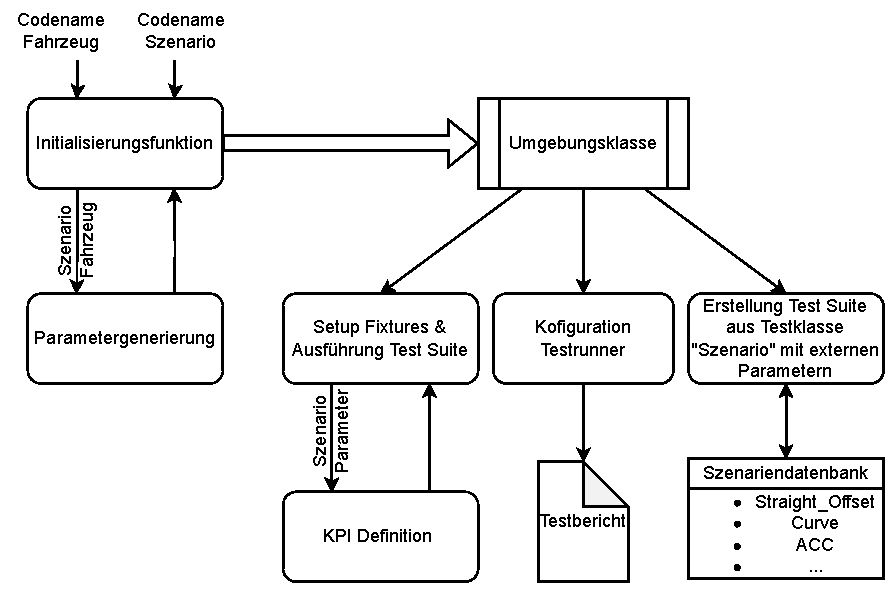
\includegraphics[width=0.9\textwidth]{figures/3_Implementierung/Ablauf_TestSkript.drawio.pdf}
    \caption{schematischer Ablauf eines Testskripts zur Ausführung eines Szenarios}
    \label{fig:Testskript_Ablauf}
\end{figure}

\subsection{Parametergenerierung} \label{subsec:Parametergenerierung}
In bisherigen Testdurchführungen wurden die Parameter für Szenarien manuell gewählt und in ein Skript geschrieben. Für eine größere Anzahl an Parametern bzw. eine größere Testabdeckung ist dieses Verfahren sehr aufwändig und deckt möglicherweise nicht den gesamten Parameterraum ab. Wie bereits in Kapitel \ref{sec:SoftwaretestsAutomobil} geschildert, ist es nicht möglich, jede Parameterkombination eines ausgewählten Szenarios abzutesten. Besitzt ein Szenario $N$ Parameter und existieren für jeden dieser Parameter $k$ verschiedene Werte, so werden bei einer vollständigen Abtestung des Parameterraums $k^{N}$ Simulationen benötigt. Die Anzahl der Simulationen steigt exponentiell mit der Anzahl der Parameter an. Vor allem bei komplexeren Szenarien ist diese Parametrierungsstrategie nicht anwendbar.

Um die Anzahl der notwendigen Simulationen zu reduzieren, wurden folgende Strategien angewendet:
\begin{itemize}
    \item sinnvolle Begrenzung des Parameterraums
    \item Implementierung einer (zufälligen) Sampling Methode
    \item Diskretisierung des Parameterraums
\end{itemize}
Die Begrenzung des Parameterraums geschieht durch das Festlegen von Ober- und Untergrenzen für Parameterwerte. Diese Grenzen können durch das verwendete Fahrzeug gegeben sein, beispielsweise minimale Lenkradien oder Höchstgeschwindigkeiten oder durch Normen festgelegt. Beispielsweise werden in \cite{Bau2019} minimale Kurvenradien bei der Anlage von Straßen beschrieben. Noch fehlende Parametergrenzen wurden durch Testen der Funktionen der aktuellen MPFC Implementierung sinnvoll festgelegt.

Die Implementierung einer Samplingmethode ermöglicht eine Reduzierung der Anzahl der benötigten Simulationen. Für jeden Parameter wird aus dem jeweiligen Wertebereich ein zufälliger Wert gezogen. Dies wird für eine vorher definierte Anzahl an Samples wiederholt. Eine gute Abdeckung des gesamten Wertebereichs kann dabei allerdings nicht garantiert werden. Eine homogenere Verteilung wird durch die Verwendung des Latin Hypercube Samplings (LHS) erreicht \cite{McKay1979}. Dabei wird der Wertebereich eines jeden Parameters in $k$ äquivalent große Teilintervalle unterteilt. Aus jedem Teilintervall wird ein Wert zufällig ermittelt. Durch eine Permutation wird zusätzlich die Reihenfolge der ermittelten Werte geändert, da sonst beim Zusammenfügen zu Samplesets alle Parameterwerte in aufsteigender Reihenfolge vorliegen würden. Nach Abschluss dieser Methode stehen $k$-Samplesets zur Verfügung, die für alle Parameter in den jeweiligen Grenzen eine gute Abdeckung des Parameterraums bieten. Ein Vergleich der Verteilung von zufälligen Samples über den gesamten Parameterraum und dem LHS ist in Abbildung \ref{fig:Random_vs_LHS} zu sehen.
\begin{figure}[ht]
    \centering
    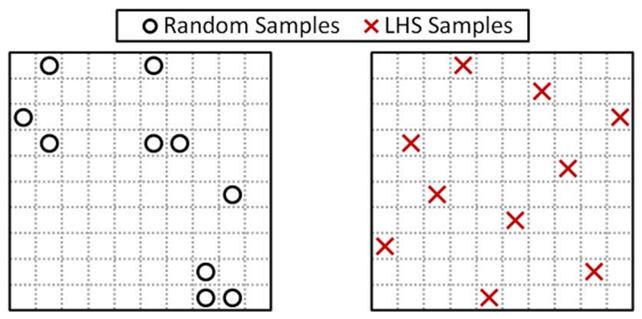
\includegraphics[width=0.5\textwidth]{figures/3_Implementierung/LHS_random_compare.png}
    \caption{Vergleich von zufälligem Sampling mit Latin Hypercube Sampling \cite{Preece2015}}
    \label{fig:Random_vs_LHS}
\end{figure}

\subsection{Definition von Key Performance Indicators und Testkriterien} \label{subsec:KPI}

Um eine Bewertung der Simulationsergebnisse vornehmen zu können, werden geeignete Daten und Grenzwerte für diese benötigt. Wird in Tests ein Über- bzw. Unterschreiten dieser festgestellt, gilt der Test als nicht bestanden. Diese Testkriterien werden als KPI bezeichnet. Ein KPI kann beispielsweise die Zeit bis zum Abbauen eines initialen lateralen Versatzes sein. Um diese zu ermitteln, werden die Pfaddaten und die tatsächliche Position des Fahrzeugs benötigt. Wird die Differenz der beiden Datensätzen nicht innerhalb der in der KPI definierten Zeitspanne abgebaut, gilt der Test als fehlgeschlagen.

Es existieren diverse Normen und Studien zur Bewertung von autonomen Fahrzeugen hinsichtlich Sicherheit und Komfort. In \cite{UNECE_R79} werden Bedingungen für die Zulassung von Fahrzeugen, welche in die Querführung des Fahrzeugs eingreifen, definiert. \cite{ISO15622} etabliert Standards für die Funktionen und Testkriterien für ein ACC-System. Weiterhin werden im Testkatalog von Euro NCAP (New Car Assessment Programme) \cite{NCAP2024}, einer Organisation, die die Sicherheit von Fahrzeugen bewertet und strenge Prüfkriterien für das Verhalten von Fahrassistenzsystemen anwendet, ebenfalls Testszenarien und Grenzwerte festgelegt. Nachfolgend wird auf die verwendeten KPIs und die Ermittlung von möglichen Grenzwerten näher eingegangen.

\bigskip\noindent\textbf{Laterale Beschleunigung}

\noindent Die laterale Beschleunigung hat großen Einfluss auf den Fahrkomfort \cite{BELLEM201890}. In \cite{ISO15622} wurde das Verhalten eines durchschnittlichen Fahrers in Kurven bei verschiedenen Geschwindigkeiten analysiert, siehe Abbildung \ref{fig:lateral_acceleration}. In \cite{UNECE_R79} werden für verschiedene Fahrzeugklassen in verschiedenen Geschwindigkeitszonen maximale Querbeschleunigungen definiert, siehe Tabelle \ref{tab:lateral_acceleration_unece}.
\begin{figure}[ht]
    \centering
    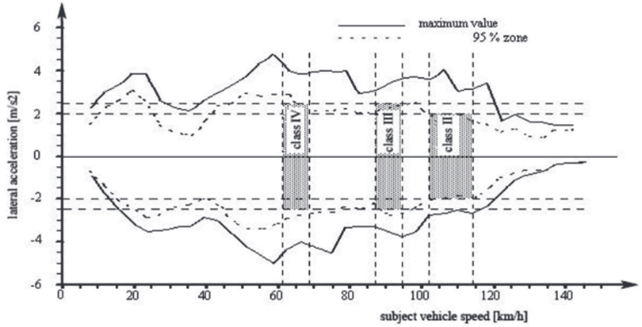
\includegraphics[width=0.8\textwidth]{figures/3_Implementierung/lateral_acceleration.png}
    \caption{laterale Beschleunigung in Kurven eines typischen Fahrers \cite{ISO15622}}
    \label{fig:lateral_acceleration}
\end{figure}
\begin{table}[H]
    \newcolumntype{C}{>{\centering\arraybackslash}m{0.115\textwidth}}
    \centering
    \caption{Höchstwerte für laterale Beschleunigung, aufgeschlüsselt nach Fahrzeugklassen und Geschwindigkeitszonen \cite{UNECE_R79}}
    \label{tab:lateral_acceleration_unece}
    \begin{tabular}{m{0.40\textwidth}|C|C|C|C}
        \multicolumn{5}{c}{Für Fahrzeuge der Klassen M1 und N1} \\ 
        \hline
        Geschwindigkeitsbereich                                    & 10-60 km/h    & > 60-100 km/h & > 100-130 km/h & > 130 km/h  \\ 
        \hline
        Höchstwert für die angegebene maximale Querbeschleunigung  & 3 $m/s^{3}$   & 3 $m/s^{3}$   & 3 $m/s^{3}$    & 3 $m/s^{3}$ \\
        \hline
        Mindestwert für die angegebene maximale Querbeschleunigung & 0 $m/s^{3}$   & 0 $m/s^{3}$   & 0 $m/s^{3}$    & 0 $m/s^{3}$ \\ 
        \hline
        \multicolumn{5}{c}{Für Fahrzeuge der Klassen M2, M3, N2 und N3} \\ 
        \hline
        Geschwindigkeitsbereich                                    & 10-30 km/h    & > 30-60 km/h  & > 60 km/h      &             \\ 
        \hline
        Höchstwert für die angegebene maximale Querbeschleunigung  & 2,5 $m/s^{3}$ & 2,5 $m/s^{3}$ & 2,5 $m/s^{3}$  &             \\ 
        \hline
        Mindestwert für die angegebene maximale Querbeschleunigung & 0 $m/s^{3}$   & 0,3 $m/s^{3}$ & 0,5 $m/s^{3}$  &             \\
        \hline
    \end{tabular}
\end{table}

\bigskip\noindent\textbf{Longitudinale Beschleunigung}

\noindent Diese KPI ist vor allem im Kontext des ACC von großer Relevanz, da auf ein vorausfahrendes Fahrzeug möglichst sanft reagiert werden sollte. In \cite{ISO15622} sind dafür Grenzwerte definiert (Abbildung \ref{fig:iso_acceleration}). Darin werden für diese Größe keine Maximalwerte, sondern der gleitende Durchschnitt über zwei Sekunden betrachtet, woran sich die Bewertung in den implementierten Tests ebenfalls orientiert.
\begin{figure}[H]
    \centering
    \hspace*{\fill}
    \begin{subfigure}[b]{.4\textwidth}
        \centering
        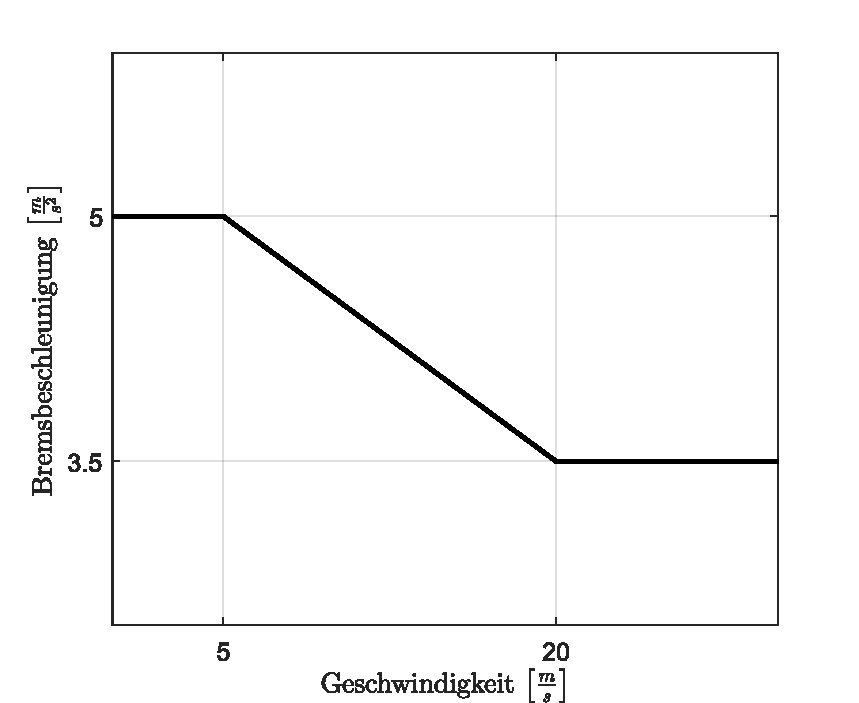
\includegraphics[width=\textwidth]{figures/3_Implementierung/max_acceleration.pdf}
        \caption{maximale Beschleunigung}
        \label{fig:max_acceleration}
    \end{subfigure}
    \hfill
    \begin{subfigure}[b]{.4\textwidth}
        \centering
        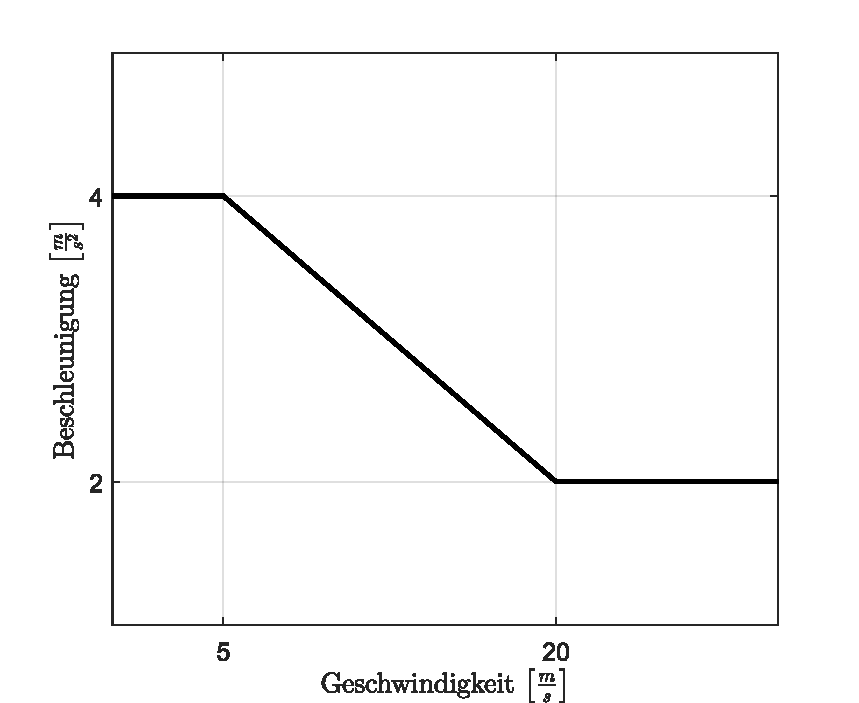
\includegraphics[width=\textwidth]{figures/3_Implementierung/max_deceleration.pdf}
        \caption{maximale Bremsbeschleunigung}
        \label{fig:max_deceleration}
    \end{subfigure}
    \hspace*{\fill}
    \caption{maximal zulässige longitudinale Beschleunigung, Durchschnitt über 2 s \cite{ISO15622}}
    \label{fig:iso_acceleration}
\end{figure}

\bigskip\noindent\textbf{Ruck}

\noindent Ruck ist ein unerwünschtes Verhalten bei Fahrzeugen, das durch ungleichmäßige Beschleunigungs- und Bremsvorgänge entsteht und maßgeblich für die Wahrnehmung von Komfort mitverantwortlich ist. \cite{ISO15622} definiert im ACC Kontext dafür einen Grenzwert für einen negativen longitudinalen Ruck, wie er beim Abbremsen entsteht. Ausgehend davon wird der auftretende laterale Ruck in den Tests betragsmäßig gesehen und entsprechend bewertet. In \cite{UNECE_R79} darf der gleitende Mittelwert des lateralen Rucks über eine halbe Sekunde nicht größer als $5\frac{m}{s^{3}}$ sein.
\begin{figure}[ht]
    \centering
    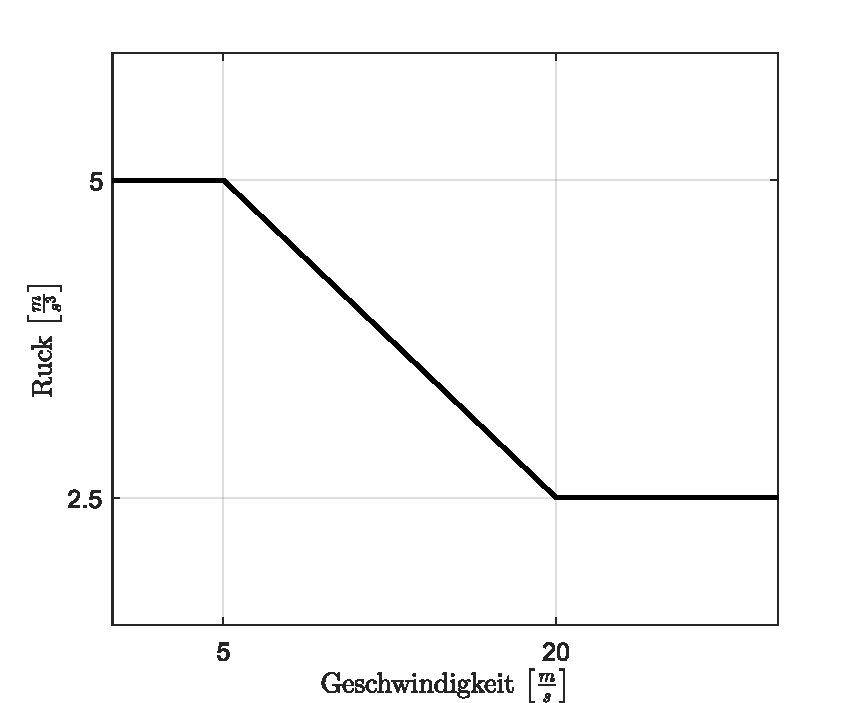
\includegraphics[width=0.4\textwidth]{figures/3_Implementierung/max_neg_jerk.pdf}
    \caption{maximal zulässiger negativer Ruck, Durchschnitt über 1 s \cite{ISO15622}}
    \label{fig:neg_jerk}
\end{figure}

\bigskip\noindent\textbf{Pfadgeschwindigkeitseinhaltung}

\noindent Die Einhaltung der vorgegebenen Pfadgeschwindigkeit ist aus Sicht der Sicherheit und der Gesetzgebung ein wichtiges Kriterium. Eine Unterschreitung ist hier weniger kritisch zu betrachten. Eine Überschreitung sollte vom System vermieden werden. Im Testkatalog von Euro NCAP wird ein System mit automatischer Geschwindigkeitsanpassung als sehr gut bewertet, wenn es die Geschwindigkeit auf $\pm2\frac{km}{h}$ anpassen kann, bevor die Frontachse des Fahrzeugs eine Zone mit niedrigerer Pfadgeschwindigkeit betritt \cite{NCAP2024}. Da die Simulation die Hinterachse als Referenz nutzt und darauf regelt, wird dieses Kriterium dahingehend angepasst.

\bigskip\noindent\textbf{Weitere KPIs}

\noindent Neben den oben genannten KPIs, welche in der Literatur gängige Anwendung finden und quantifiziert werden, wurden für die jeweiligen Szenarien weitere definiert.

\begin{itemize}
    \item \textbf{laterale Ablage} - Abweichung der Fahrzeugposition von dem gewünschten Pfad
    \item \textbf{Einschwingzeit} - benötigte Zeit, bis ein Einschwingvorgang abgeschlossen ist. Diese Zeit ist beendet, wenn die betrachtete Größe weniger als $\pm 10 \%$ vom Sollwert abweicht. 
    \item \textbf{Reaktionszeit} - benötigte Zeit, bei der eine Sprungantwort zum ersten Mal die neue Sollgröße erreicht 
    \item \textbf{Differenzgeschwindigkeit} - Geschwindigkeitsdifferenz zwischen Ego-Fahrzeug und dem ACC-Target zu einem bestimmten Zeitpunkt (abhängig vom Szenario)
    \item \textbf{Distanzfehler} - Abweichung von der gewünschten Distanz zwischen dem Ego und einem Zielobjekt zu einem bestimmten Zeitpunkt (abhängig vom Szenario)
\end{itemize}

\section{Integration in die GitLab CI Pipeline} \label{sec:CIPipeline}
Für das automatisierte Testen in der Pipeline wird eine .yaml-Datei benötigt \cite{GitLabDoks}. In dieser werden Jobs definiert. Ein Job ist die kleinste Einheit einer Pipeline und definiert eine zu erledigende Aufgabe. Eine Pipeline ist somit eine Ansammlung von zeitgleich gestarteten Jobs. Ein Job besteht mindestens aus der Ausführung eines Skriptes, ähnlich einer Kommandozeilenumgebung. Weiterhin kann definiert werden, wann ein Job gestartet wird und welche Voraussetzungen für diesen geschaffen werden müssen. Für jede Szenario- und Fahrzeugkombination kann ein Job erstellt werden. Ein Job führt zunächst Setup-Skripte aus, damit anschließend Matlab\textsuperscript{\textregistered} über eine Befehlszeileneingabe gestartet werden kann. Der Ablauf ist ähnlich zu dem in Abschnitt \ref{fig:Testskript_Ablauf} beschrieben. Es wird lediglich ein anderes Initialisierungsskript verwendet, um mit den geänderten Gegebenheiten in der Pipeline umzugehen.

\subsection{Darstellung der Pipeline}
Um die Wartung der .yaml-Datei zu vereinfachen und die Ausführung übersichtlicher zu gestalten, wird die Funktionalität von GitLab ausgenutzt, Jobs in einer Matrix zu parametrisieren. Dabei wird lediglich ein Job für jedes Fahrzeug erstellt. In diesem Job werden über den \textit{matrix} Befehl die gewünschten Szenarien, welche für dieses Fahrzeug abgetestet werden sollen, hinterlegt. Die Pipeline generiert dann automatisch für jede Kombination aus Fahrzeug und Szenario einen eigenen Job an. Durch geeignete Wahl der Testklassennamen ist es zusätzlich möglich in einem Job, mehrere Testklassen/Szenarien nacheinander laufen zu lassen. Beispielsweise wird im Job "'test\_Curve"' sowohl ein normales Kurvenfahrtszenario als auch der in Abschnitt \ref{sec:kurveNegativ} vorgestellte Negativtest für eine Kurve ausgeführt. Weiterhin können durch die Verwendung des \textit{parallel} Kennworts mehrere Jobs parallel ablaufen, was die Laufzeit der Pipeline enorm verkürzt. Durch diese Einstellung der Pipeline ergibt sich eine sehr übersichtliche Darstellung im Browser (Abbildung \ref{fig:uebersicht_pipeline}). Aus dieser ist direkt zu entnehmen, welche Szenarios für welches Fahrzeug (Alice, IAVShuttle) ausgeführt wurden und welche Szenarien zu Fehlern geführt haben.
\begin{figure}[ht]
    \centering
    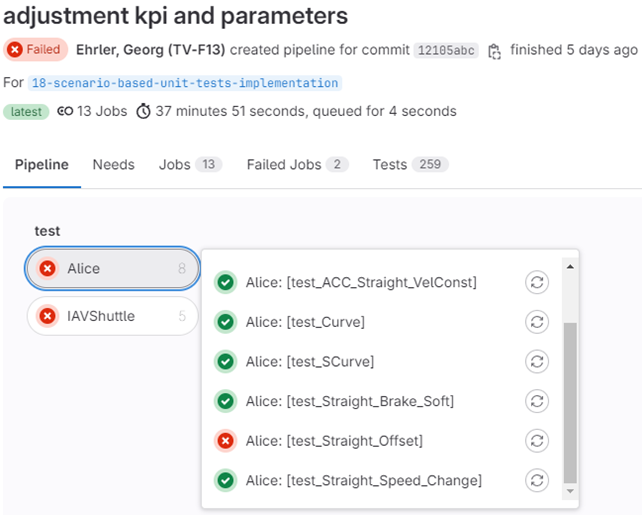
\includegraphics[width=0.6\textwidth]{figures/3_Implementierung/uebersicht_pipeline.png}
    \caption[Darstellung der Jobs in der GitLab CI Pipeline]{Darstellung der Jobs in der GitLab CI Pipeline im Browser. "'Alice"' und "'IAVShuttle"' sind Codenamen von Prototypenfahrzeugen}
    \label{fig:uebersicht_pipeline}
\end{figure}

\subsection{Darstellung der Testergebnisse}
Nachdem ein Szenario durchlaufen ist, werden die Testergebnisse sowohl in GitLab, als auch in einer PDF-Datei dargestellt. Dieser Testbericht wird als Artefakt des jeweiligen Jobs behalten und kann vom Entwickler herunterladen werden.

Auf der Startseite befindet sich eine Übersicht (Abbildung \ref{fig:testreport_aufmacher}). Schlägt ein Test fehl, gibt es einen ausführlicheren Bericht (Abbildung \ref{fig:failed_test}). Die Testdiagnose teilt dem Entwickler mit, was das Problem ist. Der Vergleich von soll KPI und tatsächlichem Ergebnis folgt darunter. Wenn es für den Test sinnvoll ist, wird ebenfalls ein Plot generiert, der den zeitlichen Verlauf von relevanten Größen über die Zeitdauer der Simulation darstellt. Die Parameter des aktuellen Szenarios werden ebenfalls angegeben, um den Test lokal reproduzieren zu können.
\begin{figure}[ht]
    \centering
    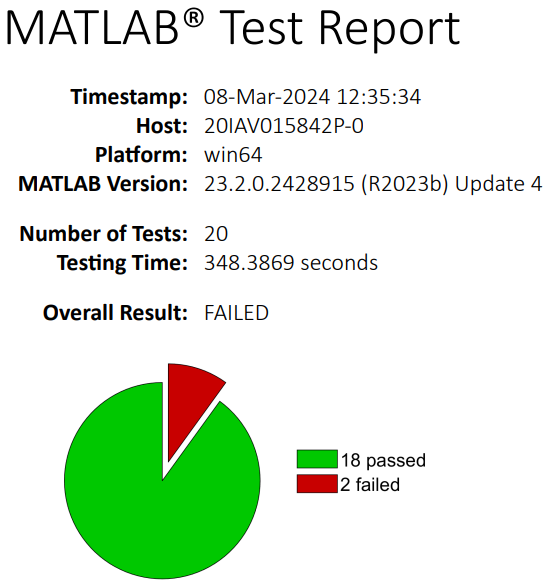
\includegraphics[width=0.45\textwidth]{figures/3_Implementierung/testreport_aufmacher.png}
    \caption[Übersichtliche Darstellung der Testergebnisse eines Szenarios]{Übersichtliche Darstellung der Testergebnisse eines Szenarios auf der ersten Seite des Testberichts}
    \label{fig:testreport_aufmacher}
\end{figure}
\begin{figure}[ht]
    \centering
    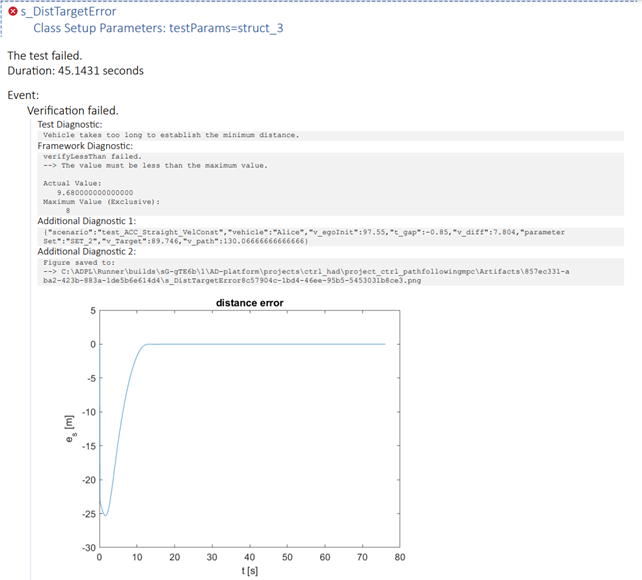
\includegraphics[width=0.8\textwidth]{figures/3_Implementierung/failed_test.png}
    \caption[Darstellung eines fehlgeschlagenen Tests im Testbericht]{Darstellung eines fehlgeschlagenen Tests im Testbericht. Der Wert der KPI und der tatsächliche Wert werden verglichen. Ein kurzer Text gibt dem Entwickler wieder, was fehlgeschlagen ist. Wenn es sinnvoll ist, wird ein Plot mit den relevanten Daten erzeugt. Die Angabe der Simulationsparameter genutzt werden, um diese eine Simulation lokal zu wiederholen.}
    \label{fig:failed_test}
\end{figure}
\chapter{Vorstellung ausgewählter Szenarien} \label{chap:Vorstellung_Szenarien}
\thispagestyle{empty}
Um geeignete Szenarien für die Simulation zu erstellen, wurden verschiedene Quellen berücksichtigt:
\begin{itemize}
    \item betriebsinterne Szenariendatenbank
    \item Normen und Richtlinien 
    \item eigene Überlegungen nach Systemanalyse
\end{itemize}
Es steht intern eine Szenariendatenbank zur Verfügung. Für diese Simulation sind viele Szenarien allerdings nicht von Relevanz, da die Pfadplanung von einem übergeordneten Modul realisiert wird und bspw. Kreuzungsszenarien zu Kurvenszenarien reduziert werden. In \cite{ISO15622} und \cite{NCAP2024} werden verschiedene Szenarien für die Einhaltung gesetzlicher Vorschriften und ACC Systeme definiert. Weiterhin wurden auch Negativtests implementiert. Dabei wird ein Szenario bewusst so parametriert, dass es der Simulation nicht möglich ist die KPIs einzuhalten. In diesen Fällen ist ein fehlschlagen eines Test als positiv zu werten. Ein Test schlägt fehl, wenn die Grenzwerte nicht überschritten wurden sind.\medskip

\noindent Im folgenden werden exemplarisch einzelne Szenarien näher erläutert. 

\section{Szenario: Gerade mit initialem Versatz} \label{sec:straight_offset}
Das Ego startet auf einer Geraden. Die Initialgeschwindigkeit ist gleich der Pfadgeschwindigkeit. Es besteht ein initialer lateraler Versatz von der Ego Position zum gewünschten Pfad. Das Ego sollte den initialen Versatz abbauen und mit der Pfadgeschwindigkeit auf dem gewünschten Pfad fahren. Die gerine Komplexität und Parameteranzahl des Szenarios ermöglichen eine einfache Analyse von Auswirkungen der Veränderung eines Parameters bei gleichzeitiger Konstanthaltung der anderen Parameter. Dafür wurde in allen Diagrammen das gleiche MPC-Parameterset und das gleiche Fahrzeug verwendet.
\begin{figure}[ht]
    \centering
    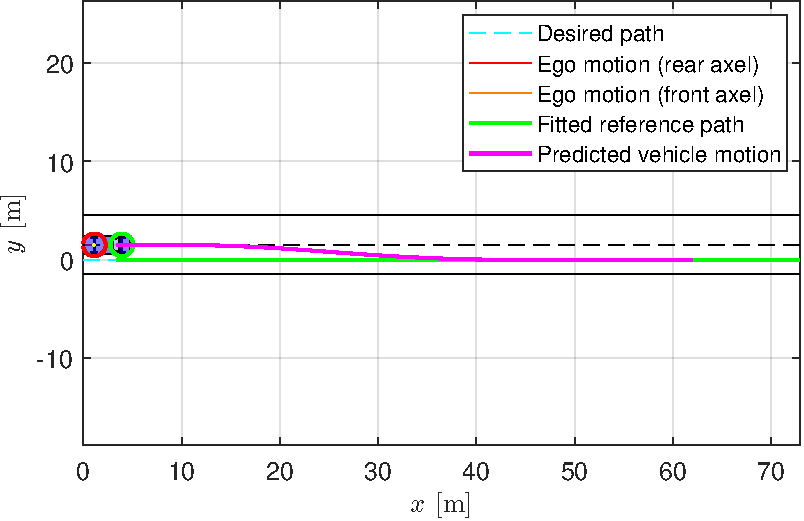
\includegraphics[width=0.5\textwidth]{figures/3_Implementierung/Straight_Offset/test_straight_depiction.pdf}
    \caption{Darstellung des Szenarios: Gerade mit initialem Versatz}
    \label{fig:test_straight_depiction}
\end{figure}

\subsection{Parametrierung}
Die Parameter für dieses Szenario sind:
\begin{itemize}
    \item Versatz $[m]$: $s_{offset} \in [-1.5,1.5]$ 
    \item Initialgeschwindigkeit $[km\cdot h^{-1}]$: $v_{Ego} \in [10,v_{vehicle,max}]$
    \item verwendetes MPC Parameterset 
\end{itemize}

\subsection{Abgetestete KPIs}
Es wurden Test für folgende KPIs mit den dazugehörigen Grenzwerten implementiert:

\medskip\noindent\textbf{Einschwingzeit:}: der laterale Versatz sollte innerhalb einer bestimmten Zeit abgebaut werden: $t_{settle} < kpi_{t_{settle}}$

\noindent Eine Variation des Versatzes bei gleicher Geschwindigkeit von 50 km/h (Abbildung \ref{fig:varOffset_50kmh_s-Error}) führt zu sehr ähnlichem Verhalten und einer nahezu identischen Reaktionszeit (erster Nulldurchlauf). Je größer der Versatz desto höher ist das Überschwingen auf der anderen Seite des Pfades, was zu einer längeren Einschwingzeit führt. Bei der Variation der Geschwindigkeit (Abbilfung \ref{fig:varVelo_1mOffset_s-Error}) und konstantem Versatz von 1 m verschiebt sich der Zeitpunkt des maximalen Überschwingens nach hinten, je geringer die Geschwindigkeit wird.  Durch die Wahl eines Grenzwertes der maximalen Pfadabweichung kann die Einschwingzeit bestimmt werden, indem das letzte Überschreiten des Grenzwertes ermittelt wird.
\begin{figure}[ht]
    \centering
    \begin{subfigure}[b]{.49\textwidth}
        \centering
        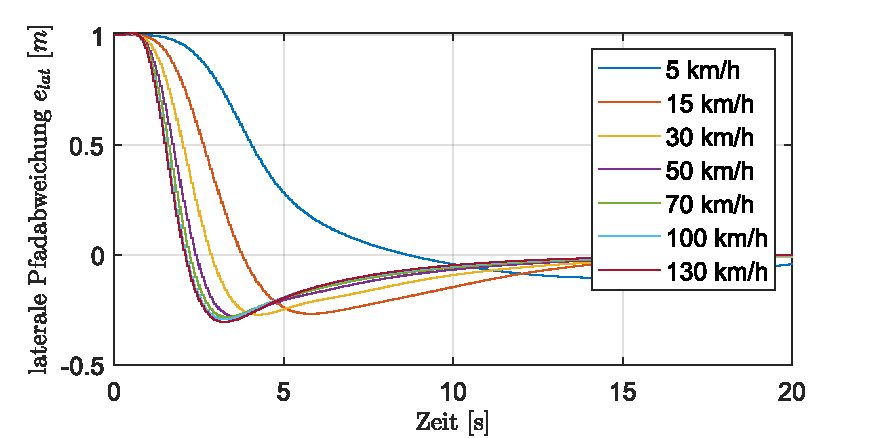
\includegraphics[width=\textwidth]{figures/3_Implementierung/Straight_Offset/varVelo_1mOffset_s-Error.pdf}
        \caption{Variation der Initialgeschwindigkeit}
        \label{fig:varVelo_1mOffset_s-Error}
    \end{subfigure}
    \hfill
    \begin{subfigure}[b]{.49\textwidth}
        \centering
        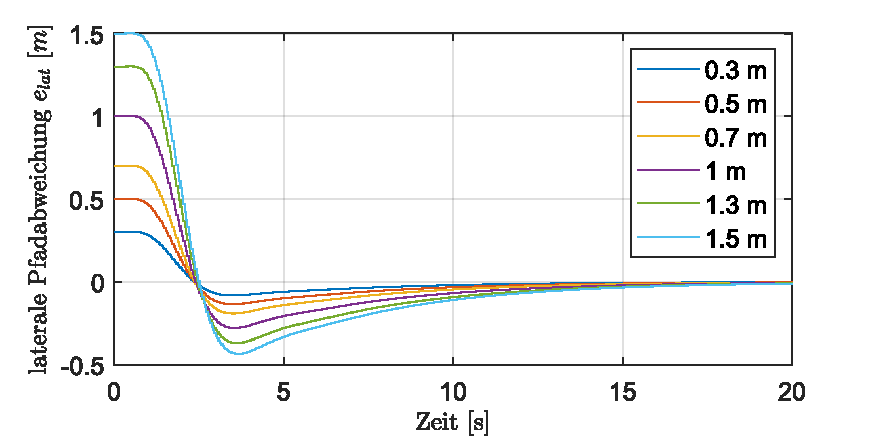
\includegraphics[width=\textwidth]{figures/3_Implementierung/Straight_Offset/varOffset_50kmh_s-Error.pdf}
        \caption{Variation des initialen Versatzes}
        \label{fig:varOffset_50kmh_s-Error}
    \end{subfigure}
    \caption{KPI Pfadabweichung abhängig der Simulationsparameter}
    \label{fig:Straight_Offset_s-Error}
\end{figure}

\medskip\noindent\textbf{longitudinale Geschwindigkeit:} die Geschwindigkeitsabweichung zum Pfad darf den Grenzwert nicht überschreiten: $|v_{Long} - v_{Path}| < kpi_{v_{diff}}$

\noindent Die Pfadgeschwindigkeit ist in der Implementierung der MPFC ein Optimierungsparameter. Ein verhindern des Überschreitens der Pfadgeschwindigkeit ist nicht garantiert. Um den Versatz möglichst schnell abzubauen beschleunigt der Regler das Fahrzeug. Dies ist vorallem bei niedrigeren Geschwindigkeiten und höheren Versätzen zu beobachten, siehe Abbildungen \ref{fig:Straight_Offset_s-Error}.   
\begin{figure}[ht]
    \centering
    \begin{subfigure}[b]{.49\textwidth}
        \centering
        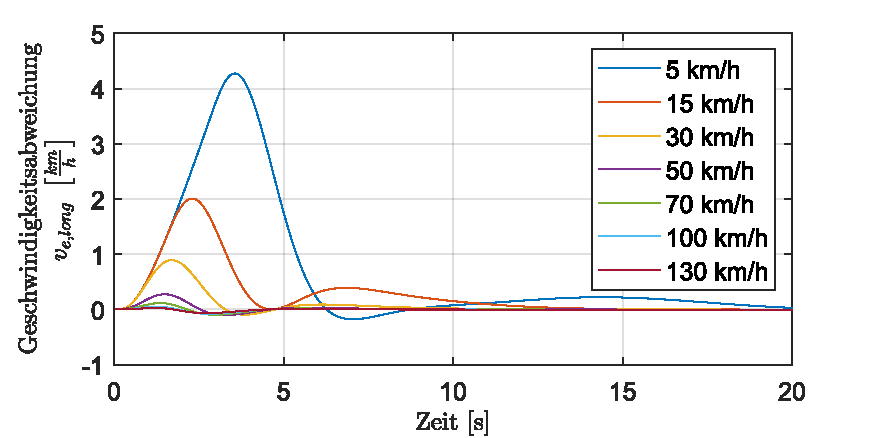
\includegraphics[width=\textwidth]{figures/3_Implementierung/Straight_Offset/varVelo_1mOffset_v-Diff.pdf}
        \caption{Variation der Initialgeschwindigkeit}
        \label{fig:varVelo_1mOffset_v-Diff}
    \end{subfigure}
    \hfill
    \begin{subfigure}[b]{.49\textwidth}
        \centering
        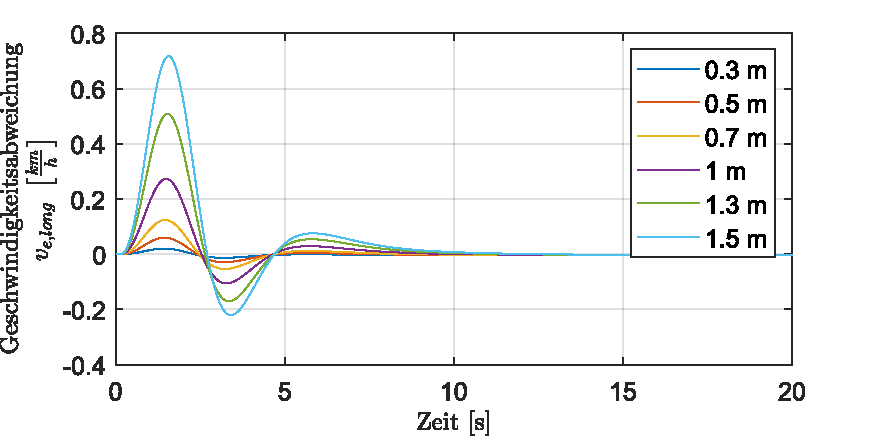
\includegraphics[width=\textwidth]{figures/3_Implementierung/Straight_Offset/varOffset_50kmh_v-Diff.pdf}
        \caption{Variation des initialen Versatzes}
        \label{fig:varOffset_50kmh_v-Diff}
    \end{subfigure}
    \caption{KPI Geschwindigkeitsabweichung abhängig der Simulationsparameter}
    \label{fig:Straight_Offset_v-Diff}
\end{figure}

\medskip\noindent\textbf{laterale Beschleunigung:} der gleitende Mittelwert über eine halbe Sekunde darf den Grenzwert nicht überschreiten: $a_{Lat} < kpi_{a_{Lat}}$

\noindent Wie aus Abbildung \ref{fig:Straight_Offset_a-Lat} hervorgeht führen höhere Geschwindigkeiten und ein größerer initialer Versatz erwartungsgemäß zu größeren Amplituden.
\begin{figure}[ht]
    \centering
    \begin{subfigure}[b]{.49\textwidth}
        \centering
        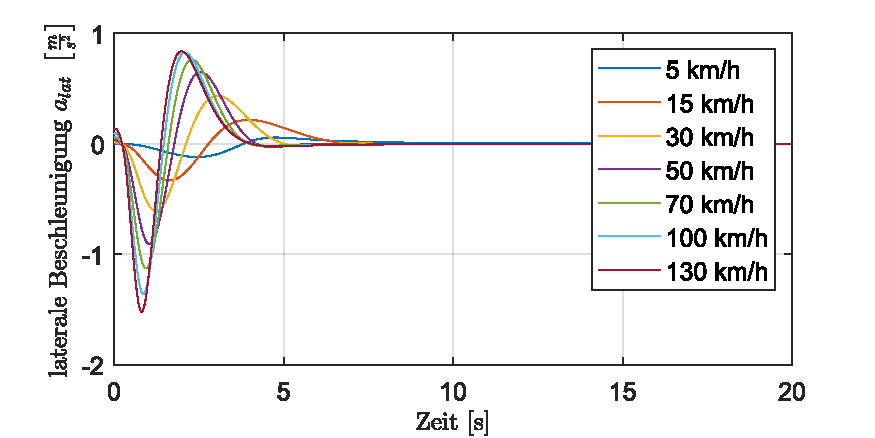
\includegraphics[width=\textwidth]{figures/3_Implementierung/Straight_Offset/varVelo_1mOffset_a-Lat.pdf}
        \caption{Variation der Initialgeschwindigkeit}
        \label{fig:varVelo_1mOffset_a-Lat}
    \end{subfigure}
    \hfill
    \begin{subfigure}[b]{.49\textwidth}
        \centering
        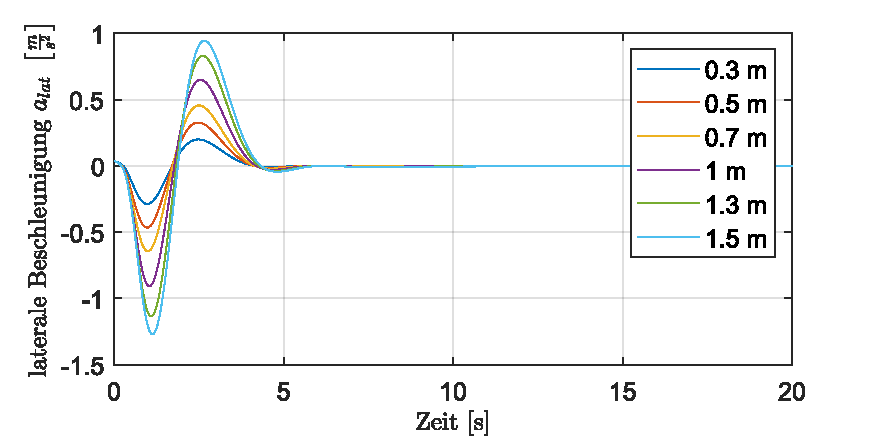
\includegraphics[width=\textwidth]{figures/3_Implementierung/Straight_Offset/varOffset_50kmh_a-Lat.pdf}
        \caption{Variation des initialen Versatzes}
        \label{fig:varOffset_50kmh_a-Lat}
    \end{subfigure}
    \caption{KPI laterale Beschleunigung abhängig der Simulationsparameter}
    \label{fig:Straight_Offset_a-Lat}
\end{figure}

\medskip\noindent\textbf{lateraler Ruck:} der Gleitende Mittelwert über eine halbe Sekunde darf den Grenzwert nicht überschreiten: $j_{Lat} < kpi_{j_{Lat}}$

\noindent Wie aus Abbildung \ref{fig:Straight_Offset_j-Lat} hervorgeht führen höhere Geschwindigkeiten und ein größerer initialer Versatz erwartungsgemäß zu größeren Amplituden.
\begin{figure}[ht]
    \centering
    \begin{subfigure}[b]{.49\textwidth}
        \centering
        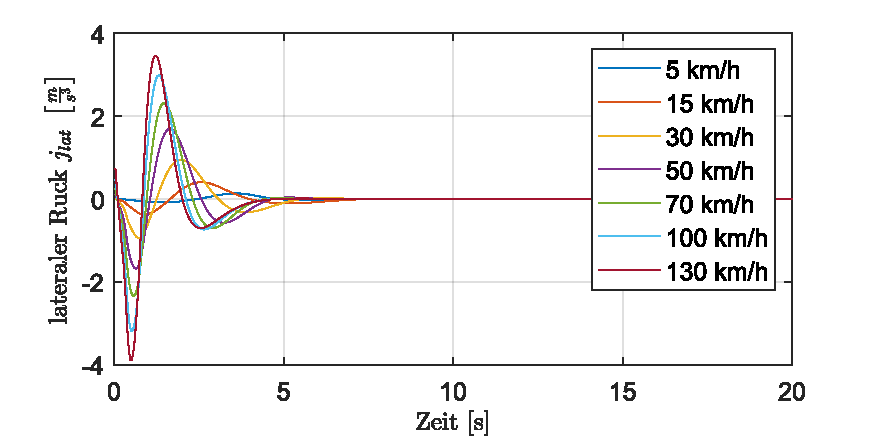
\includegraphics[width=\textwidth]{figures/3_Implementierung/Straight_Offset/varVelo_1mOffset_j-Lat.pdf}
        \caption{Variation der Initialgeschwindigkeit}
        \label{fig:varVelo_1mOffset_j-Lat}
    \end{subfigure}
    \hfill
    \begin{subfigure}[b]{.49\textwidth}
        \centering
        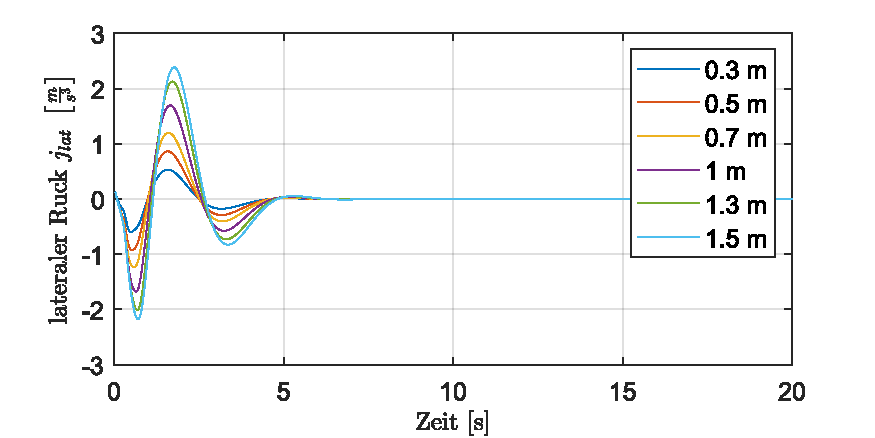
\includegraphics[width=\textwidth]{figures/3_Implementierung/Straight_Offset/varOffset_50kmh_j-Lat.pdf}
        \caption{Variation des initialen Versatzes}
        \label{fig:varOffset_50kmh_j-Lat}
    \end{subfigure}
    \caption{KPI lateraler Ruck abhängig der Simulationsparameter}
    \label{fig:Straight_Offset_j-Lat}
\end{figure}

\section{Szenario: Kurve negativ} \label{sec:kurveNegativ}
Das Ego startet mit einer Initialgeschwindigkeit, welche der Pfadgeschwindigkeit entspricht auf einer Geraden. An die Gerade schließt sich eine Kurve an, welche in einen Kreis endet. Der Radius des Kreises ist kleiner als der minimale Wendekreis des Fahrzeugs. Das Ego soll die Beschränkungen des Lenkeinschlags nicht verletzen. Dies führt dazu, dass das Fahrzeug die Kurve nicht schaffen kann und der Abstand zum gewünschten Pfad zu groß wird.
\begin{figure}[ht]
    \centering
    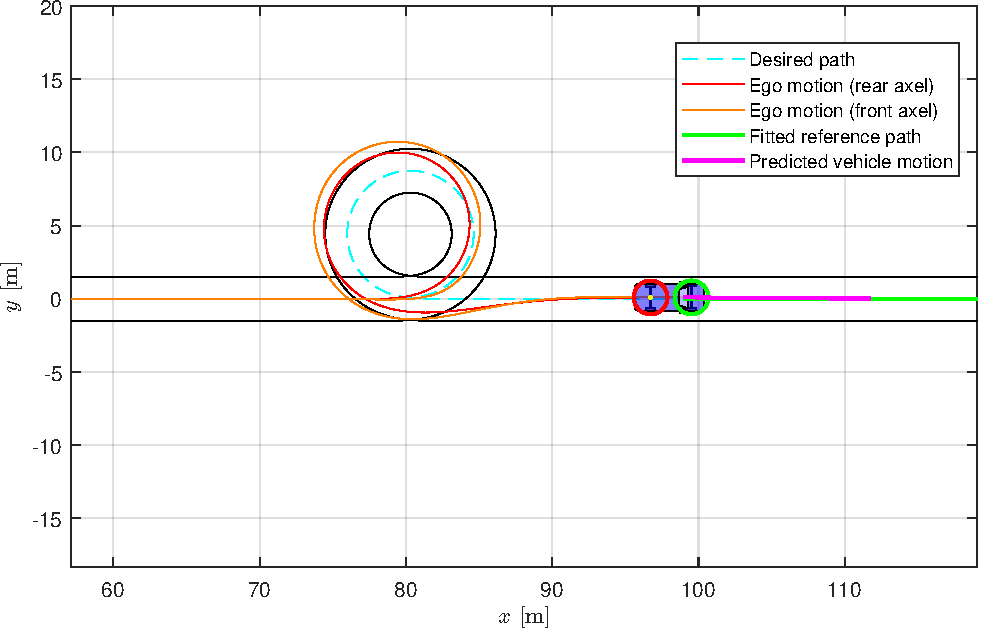
\includegraphics[width=0.5\textwidth]{figures/3_Implementierung/Curve_negative/test_curve_negative_depiction.pdf}
    \caption{Darstellung des Szenarios: Kurvenfahrt negativ}
    \label{fig:test_curve_negative_depiction}
\end{figure}

\subsection{Parametrierung}
Die Parameter für dieses Szenario sind:
\begin{itemize}
    \item maximale Querbeschleunigung in der Kurve $[m\cdot s^{-2}]$: $a_{Lat} \in [1,4]$
    \item Kurvenradius $[m]$: $s_{radius} \in [0.7,0.9]\cdot r_{min,turn}$
    \item verwendetes MPC Parameterset
\end{itemize}

\subsection{abgetestete KPIs}
Es wurden Test für folgende KPIs mit den dazugehörigen Grenzwerten implementiert:

\medskip\noindent\textbf{laterale Ablage:} die Abweichung des Fahrzeugs vom gewünschten Pfad muss größer sein als ein definierter Grenzwert: $s_{error,lat} > kpi_{s_{error,lat}}$

\noindent Wie erwartet führen kleinere Kurvenradien zu größeren maximalen Pfadabweichungen, Abbildung \ref{fig:Curve_negative_s-Error}. Nachdem die Kurve durchfahren ist kann dieser Fehler wieder abgebaut werden.
\begin{figure}[ht]
    \centering
    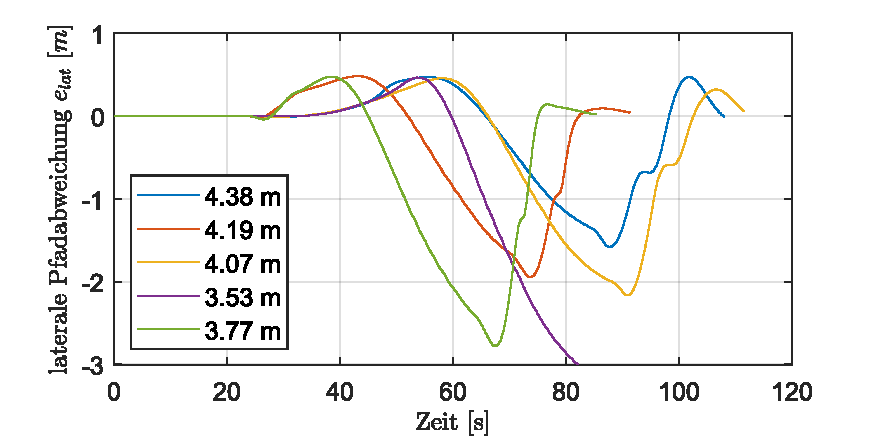
\includegraphics[width=0.5\textwidth]{figures/3_Implementierung/Curve_negative/Curve_negative_s-Error.pdf}
    \caption{KPI Pfadabweichung bei verschiedenen Kurvenradien}
    \label{fig:Curve_negative_s-Error}
\end{figure}

\section{Szenario: ACC mit konstanter Objektgeschwindigkeit} \label{sec:acc_vel_const}
Das Ego startet mit einer Initialgeschwindigkeit auf einer Geraden. Ein Target fährt vor dem Ego mit konstanter Geschwindigkeit. Es exisitiert eine Geschwindigkeitsdifferenz zwischen Ego und Target. Ebenfalls kann die initiale Zeitlücke abweichend von der gewünschten Zeitlücke sein. Das Ego sollte die Geschwindigkeitsdifferenz beseitigen und die gewünschte Zeitlücke herstellen.
\begin{figure}[ht]
    \centering
    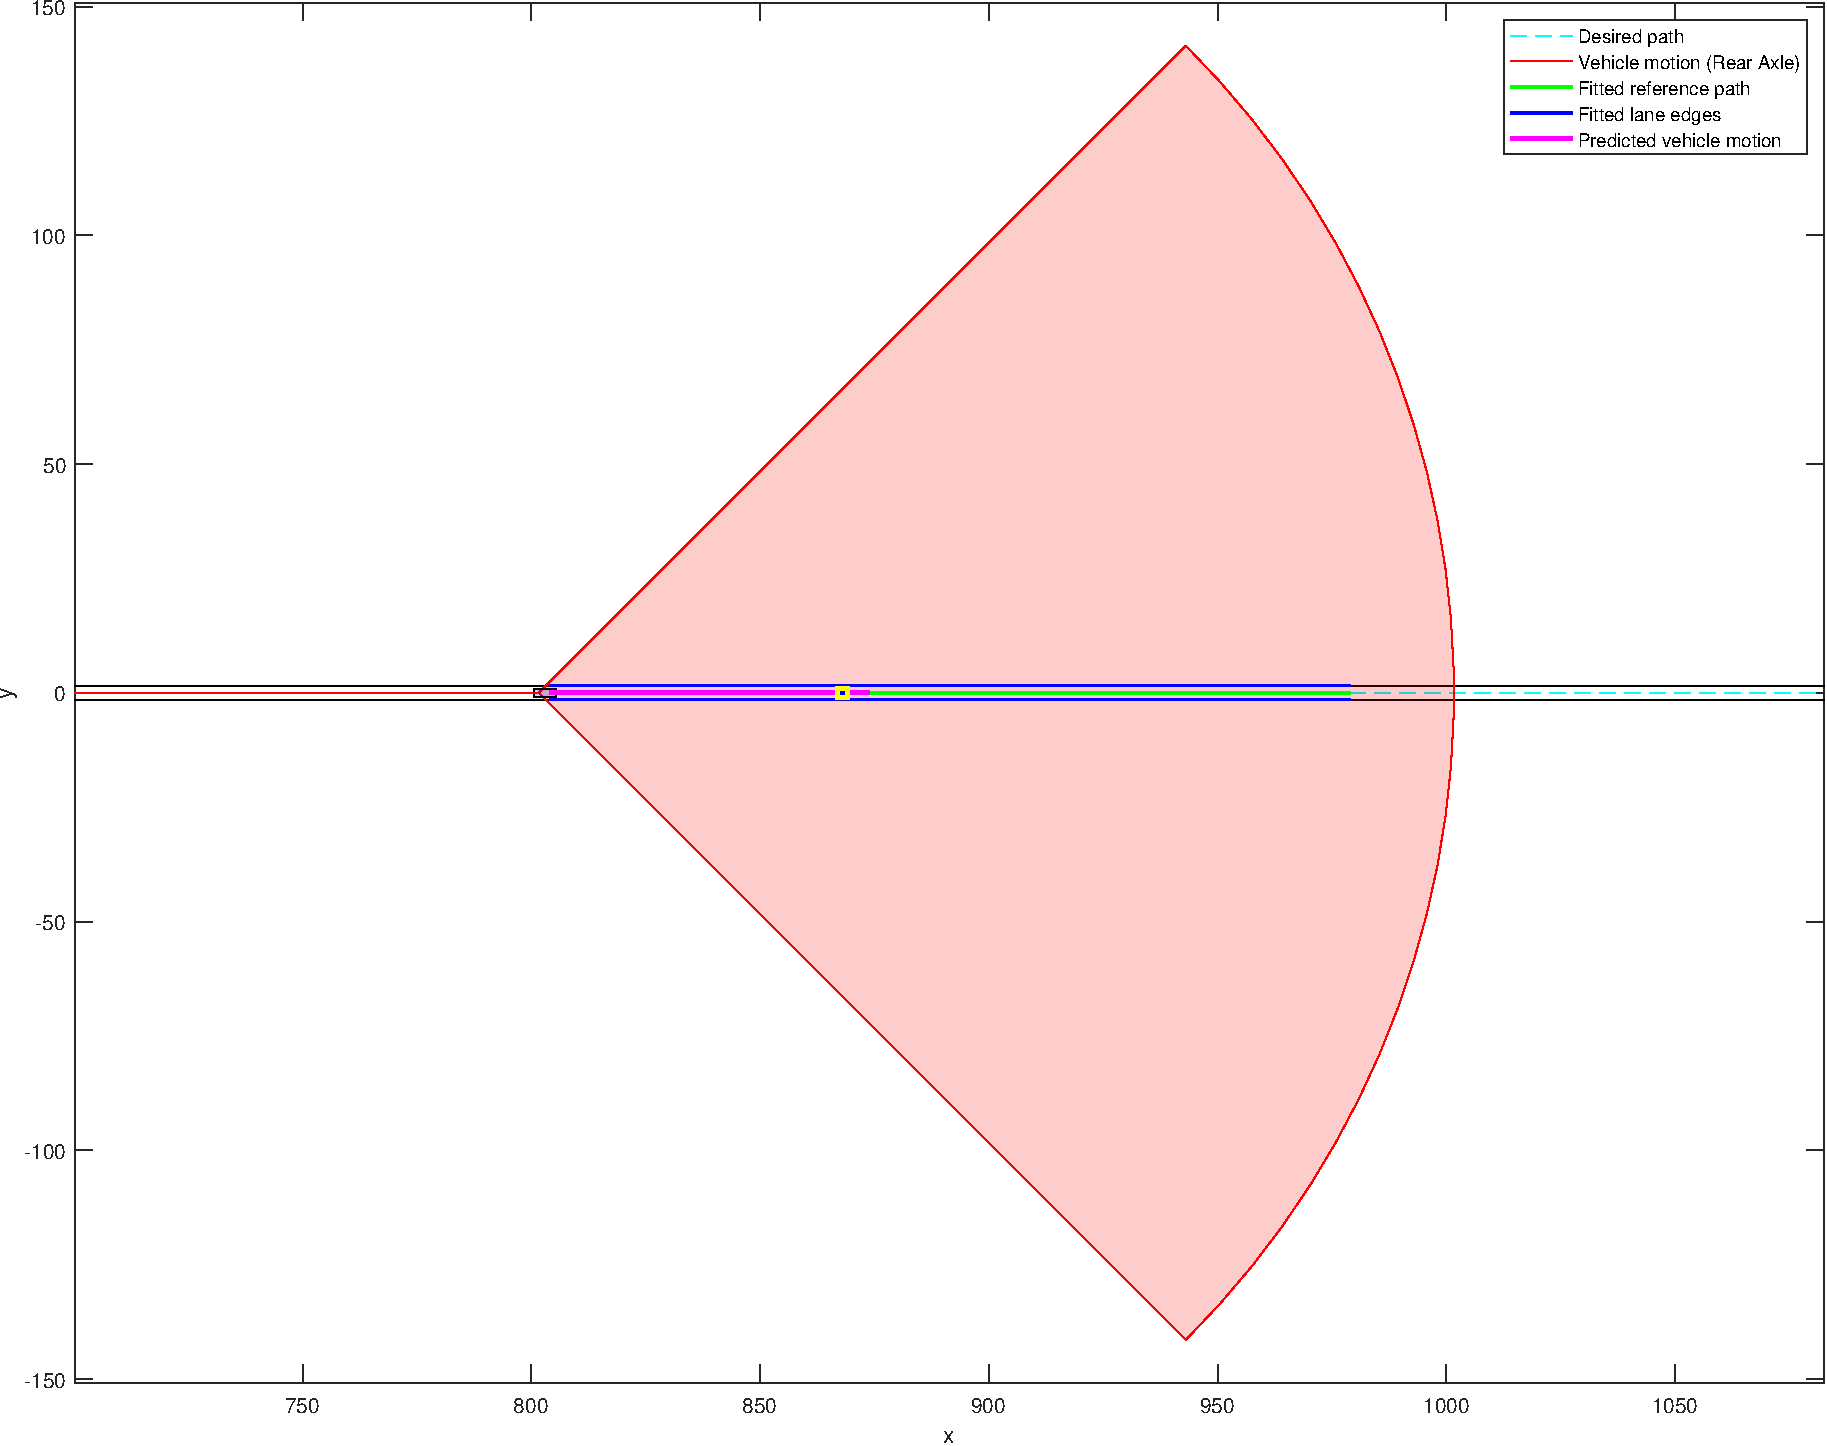
\includegraphics[width=0.5\textwidth]{figures/3_Implementierung/ACC_Vel_Const/test_ACC_Vel_Const_depiction.pdf}
    \caption{Darstellung des Szenarios: ACC mit konstanter Objektgeschwindigkeit}
    \label{fig:test_ACC_Vel_Const_depiction}
\end{figure}

\subsection{Parametrierung}
Die Parameter für dieses Szenario sind:
\begin{itemize}
    \item Initialgeschwindigkeit $[km\cdot h^{-1}]$: $v_{Ego} \in [0.2\cdot v_{vehicle,max}, 0.8\cdot v_{vehicle,max}]$
    \item Differenzgeschwindigkeit $[km\cdot h^{-1}]$: $v_{diff} \in [-0.2,0.2]\cdot v_{Ego}$
    \item Zeitlückenabweichung $[s]$: $t_{offset} \in [-1,1] + t_{gap,desired}$
    \item verwendetes MPC Parameterset
\end{itemize}

\subsection{Abgetestete KPIs}
Es wurden Test für folgende KPIs mit den dazugehörigen Grenzwerten implementiert:

\medskip\noindent\textbf{longitudinale Beschleunigung:} der Gleitende Mittelwert über eine halbe Sekunde darf einen definierten Grenzwert nicht überschreiten: $a_{Long} < kpi_{a_{Long}}$

\medskip\noindent\textbf{longitudinaler Ruck:} der Gleitende Mittelwert über eine halbe Sekunde darf den Grenzwert nicht überschreiten: $j_{Long} < kpi_{j_{Long}}$

\noindent Auftretende longitudinale Rücke und Beschleunigungen sind stark abhängig von der gewählten Paramtrierung. Eine Verletzung der Grenzwerte ist hier nicht zulässig. Vorallem darf die maximale Beschleunigung nicht größer sein als ein definierter Grenzwert. Sowohl Beschleunigung als auch Ruck befinden sich in einem akzeptablem Rahmen, siehe Abbildung \ref{fig:ACC_KPI_a_j}.

\begin{figure}[ht]
    \centering
    \begin{subfigure}[b]{.49\textwidth}
        \centering
        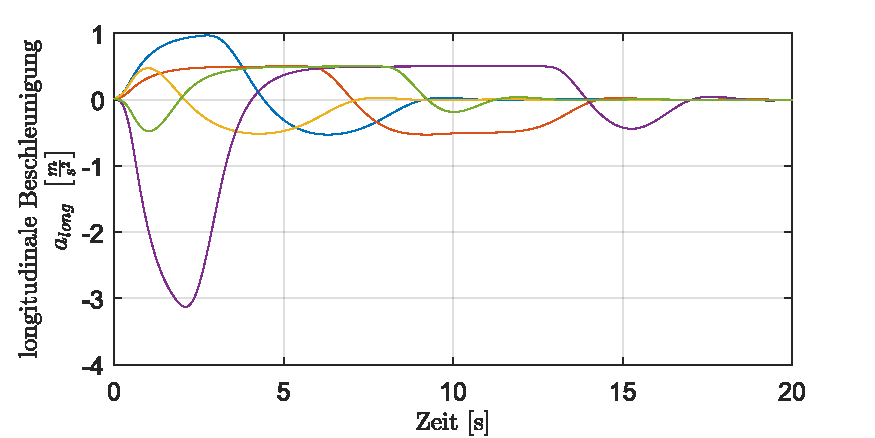
\includegraphics[width=\textwidth]{figures/3_Implementierung/ACC_Vel_Const/ACC_Vel_Const_a-Long.pdf}
    \end{subfigure}
    \hfill
    \begin{subfigure}[b]{.49\textwidth}
        \centering
        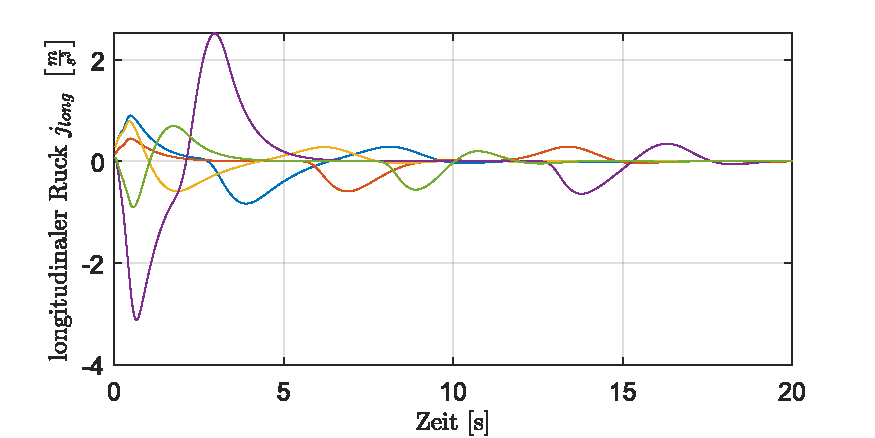
\includegraphics[width=\textwidth]{figures/3_Implementierung/ACC_Vel_Const/ACC_Vel_Const_j-Long.pdf}
    \end{subfigure}
    \caption{Simulationsdaten für Abstands- und Distanzfehler bei unterschiedlichen Parametrierungen}
    \label{fig:ACC_KPI_a_j}
\end{figure}

\medskip\noindent\textbf{Einschwingzeit:} der gewünschte Abstand zum Target sollte innerhalb einer definierten Zeit eingestellt werden: $t_{settle} < kpi_{t_{settle}}$

\noindent Durch ein optimales Systemverhalten kann die Einschwingzeit deutlich veringert werden. Allerdings ist die Definition eines festen Grenzwertes nicht möglich, da diese stark Parametrierungsabhängig ist (Abbildung \ref{fig:ACC_KPI_s_v}). 

\medskip\noindent\textbf{Reaktionszeit:} der Minimalabstand zum Target soll innerhalb einer definierten Zeit hergestellt werden: $t_{reaction} < kpi_{t_{reaction}}$

\noindent Das schnelle einstellen des Mindestabstandes ist wichtiger als die korrekte Abstandseinstellung, weswegen hier ein kürzeres Zeitfenster gewählt wurde.
\begin{figure}
    \centering
    \begin{subfigure}[b]{.49\textwidth}
        \centering
        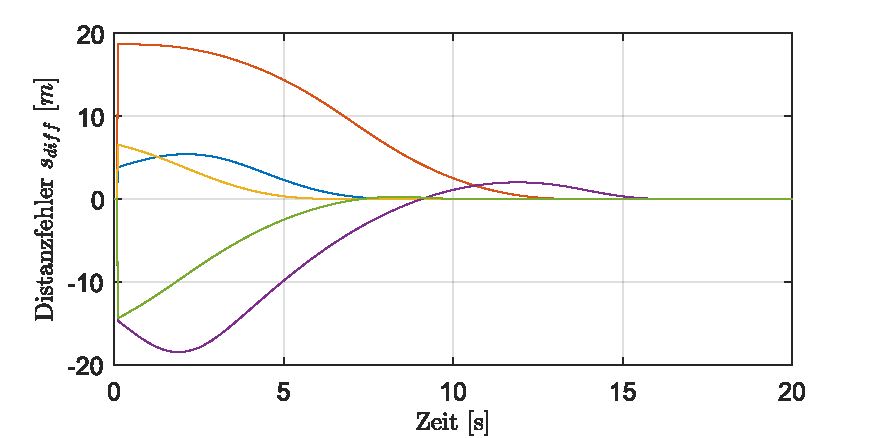
\includegraphics[width=\textwidth]{figures/3_Implementierung/ACC_Vel_Const/ACC_Vel_Const_s-Diff.pdf}
    \end{subfigure}
    \hfill
    \begin{subfigure}[b]{.49\textwidth}
        \centering
        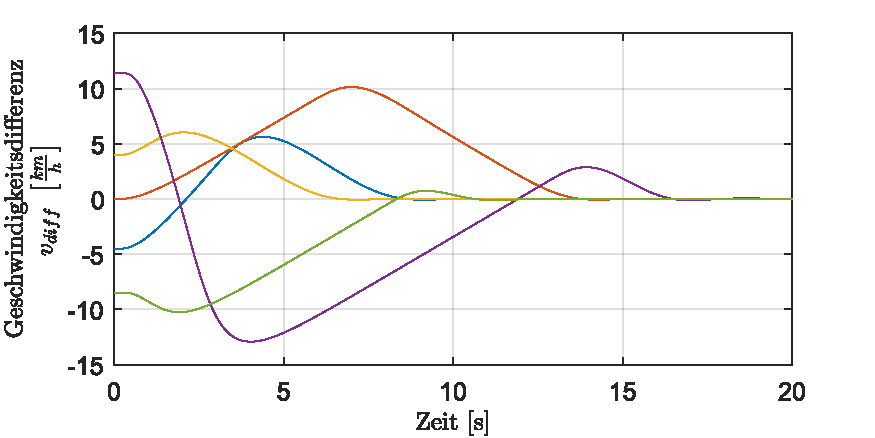
\includegraphics[width=\textwidth]{figures/3_Implementierung/ACC_Vel_Const/ACC_Vel_Const_v-Diff.pdf}
    \end{subfigure}
    \caption{Simulationsdaten für longitudinale Beschleunigung und Ruck bei unterschiedlichen Parametrierungen}
    \label{fig:ACC_KPI_s_v}
\end{figure}
\chapter{Zusammenfassung und Ausblick} \label{chap:Zusammenfassung}
\thispagestyle{empty}

Nachdem in der Einleitung die Einordnung und Vorstellung des Themas erfolgte, wurde im Grundlagenkapitel auf die zu testende Architektur eingegangen und eine theoretische Hinführung zum Thema des szenariobasierten Testen gegeben und die Relevanz von Softwaretest über den gesamten Produktlebenszyklus verdeutlicht.

Nach einer Anforderungsdefinition wurden die Möglichkeiten, die des MATLAB\textsuperscript{\textregistered} Unit Test Framework für die Umsetzung der Aufgabe bietet, ergründet und daraus ein geeignetes Konzept zur Implementierung erarbeitet. Es ermöglicht die einfache Parametrierung von Szenarien und abtesten von KPIs. Neue Szenarien können durch das Anlegen einer neuen Testklasse, Definition von KPIs und Paramertern hinzugefügt werden und müssen im jeweiligen Job für ein Fahrzeug ergänzt werden. Sollten in zukünftigen Entwicklungen weitere Fahrzeuge hinzukommen ist lediglich ein neuer Job in der .yaml-Datei für die GitLab Pipeline anzulegen. 

Nach Analyse der Simulationsumgebung und einer Literaturrecherche wurden ausgewählte Szenarien und die dazugehörigen KPIs implementiert. Um aus den ermittelten funktionalen Szenarien konkrete Szenarien zu generieren wurde das Latin Hypercube Sampling verwendet. Eine zukünftige Verbesserung dieser Sampling-Methode hinsichtlich der Generierung von kritischeren Parameterkombinationen ist denkbar. Derzeit wird, z. B. bei der Kurvenradien, aquidistant über den gesamten Parameterbereich gesampelt. Enge Kurven sind allerdings deutlich kritischer als weite Kurven, weswegen eine engere Abtastung bei kleineren Radien sinnvoller ist. Eine Möglichkeit der Umsetzung dieser Anforderung ist die Äquivalenzklassenbildung. Dabei werden für jeden Parameter Bereiche gesucht, in denen das erwartete Systemverhalten gleich ist. Es wird nun so gesampelt, dass entweder aus jeder Äquivalenzklasse genau ein Wert gebildet wird, analog zum LHS, oder aber die Anzahl an Samples in jeder Aquivalenzklasse gleich groß ist.

Die automatisierte Ausführung der Testskripte und Testklassen in einer CI Pipeline wurde erreicht. Die Testergebnisse werden übersichtlich in ein PDF-Datei verpackt oder können über den Browser im GitLab angezeigt werden. Die Testberichte geben dem Entwickler einen guten Überblick, welche Szenarien fehlgeschlagen sind und warum.
% Bibliography

\label{app:bibliography} % Reference the bibliography elsewhere with \autoref{app:bibliography}

\manualmark % Work-around to have small caps also here in the headline
\markboth{\spacedlowsmallcaps{\bibname}}{\spacedlowsmallcaps{\bibname}} % Work-around to have small caps also
%\phantomsection
\cleardoublepage % fix counter for next added section
\refstepcounter{dummy}

\addtocontents{toc}{\protect\vspace{\beforebibskip}} % Place the bibliography slightly below the rest of the document content in the table of contents
\addcontentsline{toc}{chapter}{\tocEntry{\bibname}}

\printbibliography

% \appendix
\chapter{Anhang}
\thispagestyle{empty}

\section{Test 1}

\section{Test 2}


%----------------------------------------------------------------------------------------
%	STATEMENT OF AUTHORSHIP
%----------------------------------------------------------------------------------------
\cleardoublepage
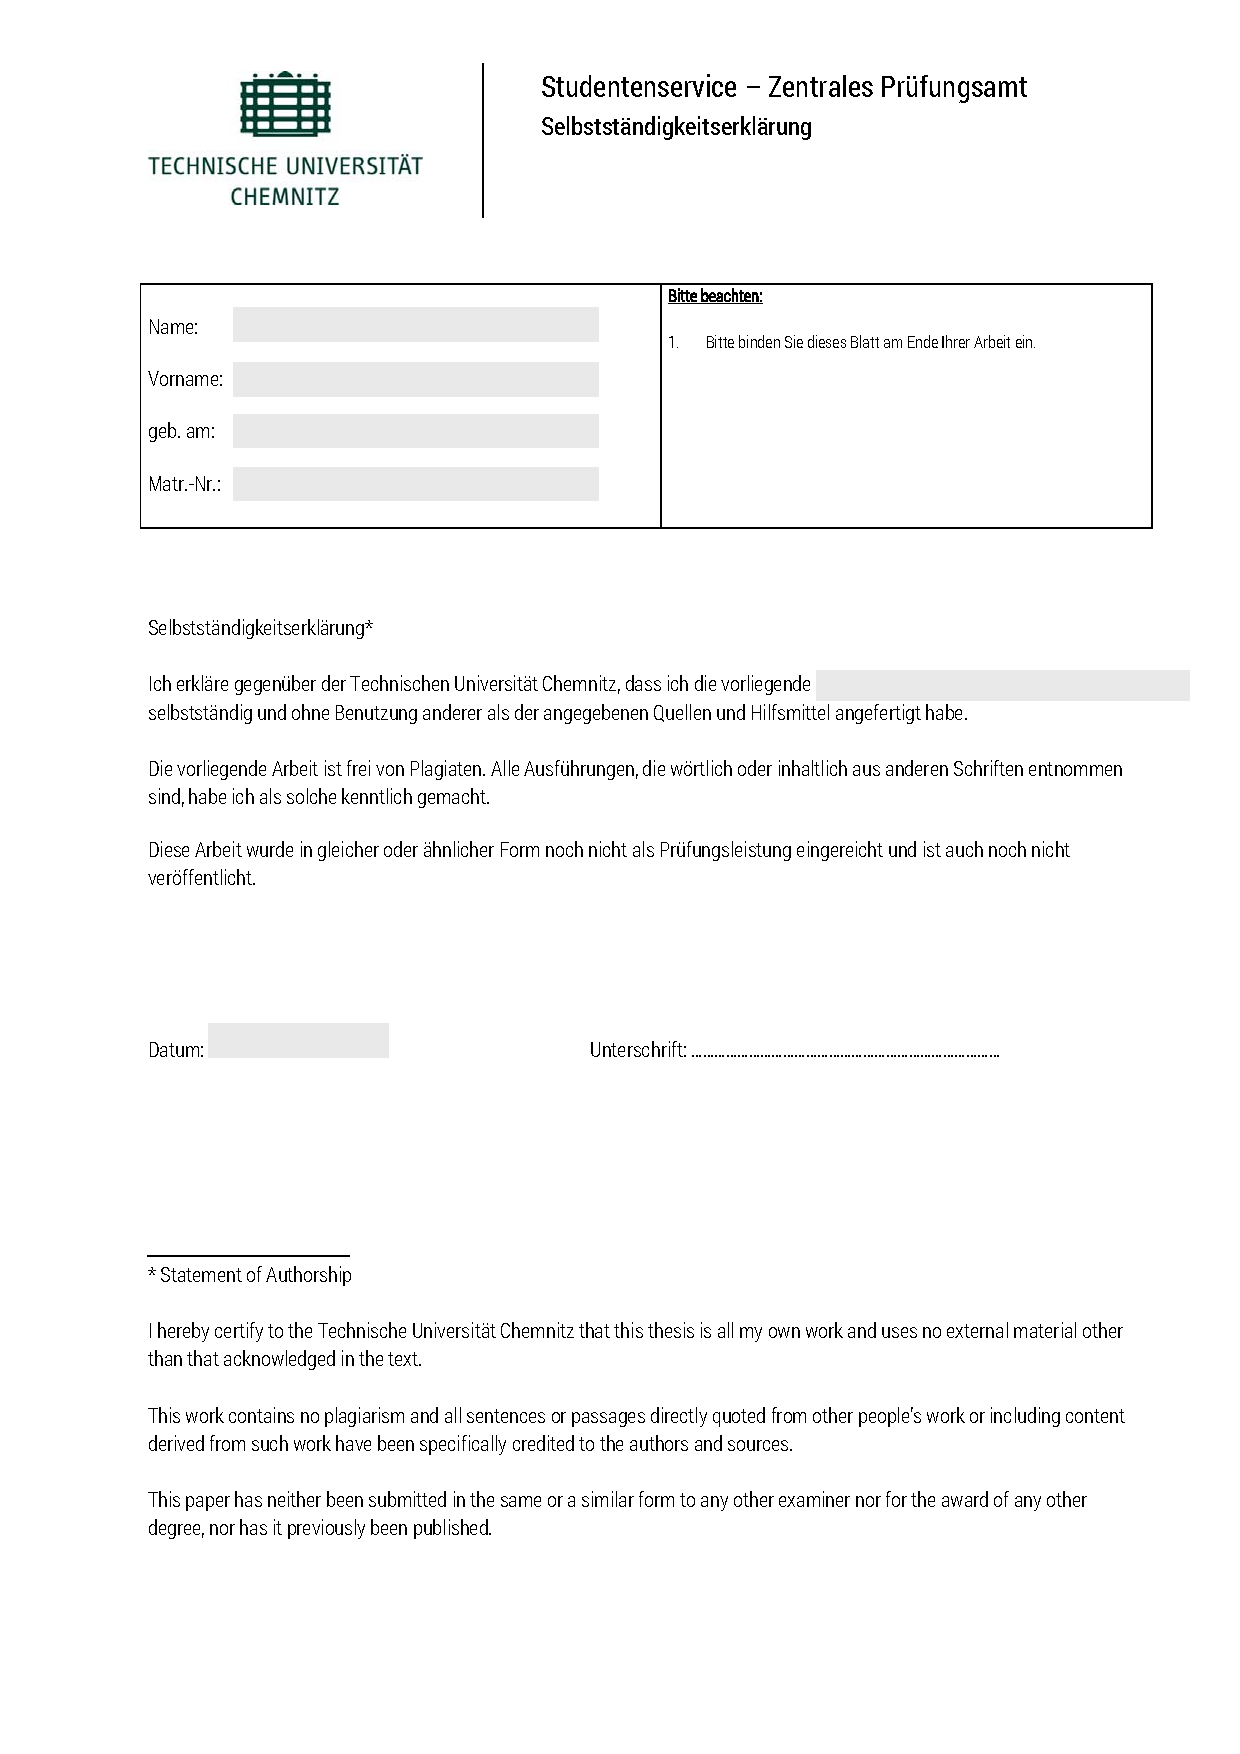
\includepdf[pages=-]{99_Authorship/selbststaendigkeitserklaerung} 
\cleardoublepage
\end{document}
